\documentclass[a4paper,32pt]{article}
\usepackage[utf8]{inputenc}
\usepackage[T1]{fontenc}
\usepackage{graphicx}
\usepackage[main=french]{babel}
\usepackage{mathptmx}
\usepackage[32pt]{moresize}
\usepackage{anyfontsize}
\usepackage{t1enc}
\usepackage{mathrsfs}
\usepackage{boldline,multirow,tabularx,colortbl,diagbox,makecell,fancybox}
\usepackage{dsfont}
\usepackage{mathtools}
\usepackage{amsfonts,amssymb,amsmath,mathrsfs,array,stmaryrd}
\usepackage{amsthm}
\usepackage{pgf,tikz,xcolor}
\usepackage{caption}
\usepackage[rightcaption]{sidecap}
\usepackage{listings}
\newcommand{\mc}[3]{\multicolumn{#1}{#2}{#3}}
\usetikzlibrary{calc,positioning,shapes.geometric,shapes.symbols,shapes.misc, fit, shapes, arrows, arrows.meta}
\usepackage[top=2.5cm, bottom=2.5cm, left=2.25cm, right=2.25cm]{geometry}
\usepackage{setspace}
\usepackage{fancyhdr}
\usepackage{indentfirst}
\usepackage{hyperref}
\theoremstyle{definition}
\newtheorem{definition}{Définition}[section]
\theoremstyle{remark}
\newtheorem{remark}{Remarque}
\theoremstyle{remarkfonda}
\newtheorem{remarkfonda}{Remarque fondamentale}
\theoremstyle{interpretation*}
\newtheorem{interpretation*}{Interprétation}
\theoremstyle{rappel}
\newtheorem{rappel}{Rappel}
\newtheorem{conclusion}{Conclusion}
\theoremstyle{proposition}
\newtheorem{proposition}{Proposition}
\theoremstyle{theorem}
\newtheorem{theorem}{Théorème}
\newtheorem{corollary}{Corollaire}
\newtheorem{lemma}[theorem]{Lemme}
\theoremstyle{example}
\newtheorem{example}{Exemple}[section]
\newenvironment{pruf}[1][Preuve]{\textit{#1:\\}}{\ \rule{0.5em}{0.5em}}
%\usepackage[svgnames]{xcolor}
\DeclareMathOperator{\sign}{sign}
\usepackage{lipsum}
\usepackage{subfig}
\usepackage{xspace,color}
\usepackage{url}
\usepackage{listings}
\lstset{commentstyle=\color{red},keywordstyle=\color{black},
showstringspaces=false}
\lstnewenvironment{rc}[1][]{\lstset{language=R}}{}
\newcommand{\ri}[1]{\lstinline{#1}}  %% Short for 'R inline'

\lstset{language=R}             % Set R to default language
%\lstset{language=R,
%basicstyle=\scriptsize\ttfamily,
%commentstyle=\ttfamily\color{gray},
%numbers=left,
%numberstyle=\ttfamily\color{gray}\footnotesize,
%stepnumber=1,
%numbersep=5pt,
%backgroundcolor=\color{white},
%showspaces=false,
%showstringspaces=false,
%showtabs=false,
%frame=single,
%tabsize=2,
%captionpos=b,
%breaklines=true,
%breakatwhitespace=false,
%title=\lstname,
%escapeinside={},
%keywordstyle={},
%morekeywords={}
%}

%==[DO NOT CHANGE ANYTHING HERE]====================
\newcommand{\addstudent}[3]{\small{#1} & \small{#2} & \small{\href{mailto:#3}{#3}}\\}
\newcommand{\addtutor}[2]{#1 & #2\\}
%==[DO NOT CHANGE ANYTHING BEFORE THIS LINE]====================

% Your PIR project title here
\def\projecttitle{
    Simulation de variables aléatoires
}

% Your keywords here
\def\varkeywords{
    Keyword 1; Keyword 2; Keyword 3; Keyword 4; Keyword 5 
}

% Your names here
\def\students{
    \addstudent{Tigzirine}{Suliman}{suliman.tigzirine@um6p.ma}
    \addstudent{Lechguar}{Yassine}{yassine.lechguar@um6p.ma}
    \addstudent{BADIDI}{Amine}{amin.badidi@um6p.ma}
    %\addstudent{Name}{SURNAME}{name.surname@mail.com}
   % \addstudent{Name}{SURNAME}{name.surname@mail.com}
}

% Your tutors here
\def\tutors{
    \addtutor{Name}{SURNAME}
   % \addtutor{Name}{SURNAME}
}

\newcommand\tab[1][0.6cm]{\hspace*{#1}} %Create and define tab


%Chapter No Numbering but appears in TOC
\newcommand{\chapternn}[1]{\chapter*{#1}\addcontentsline{toc}{chapter}{#1}}
\newcommand{\sectionnn}[1]{\section*{#1}\addcontentsline{toc}{section}{#1}}
\newcommand{\subsectionnn}[1]{\subsection*{#1}\addcontentsline{toc}{subsection}{#1}}
\newcommand{\subsubsectionnn}[1]{\subsubsection*{#1}\addcontentsline{toc}{subsubsection}{#1}}

\newcolumntype{L}[1]{>{\raggedright\arraybackslash\hspace{0pt}}p{#1}}
\newcolumntype{R}[1]{>{\raggedleft\arraybackslash\hspace{0pt}}p{#1}}
\newcolumntype{C}[1]{>{\centering\arraybackslash\hspace{0pt}}p{#1}}

\renewcommand\thesection{\arabic{section}}
\renewcommand\thesubsection{\thesection.\arabic{subsection}}


\RequirePackage{fancyhdr}
\pagestyle{fancy}

%------- Do not append new commands after :

\hypersetup{	
    colorlinks  = false, % colorise les liens
    linkbordercolor = {1 1 1},
    breaklinks  = true, % permet le retour à la ligne dans les liens trop longs
    urlcolor    = blue, % couleur des hyperliens 
    linkcolor   = black,	% couleur des liens internes 
    citecolor   = black,	% couleur des références 
    pdftitle    = {Security assessment of connected objects in the Internet of Things : State of the art}, % informations apparaissant dans 
    pdfauthor   = {}, % les informations du document 
    pdfsubject  = {}	% sous Acrobat. 
}
\title{\vspace{1.5cm}État de l'art \\ \vspace{0.25cm} \LARGE{\textbf{\projecttitle}}}
\author{}
\date{\today}
\RequirePackage{fancyhdr}
\pagestyle{fancy}
\renewcommand{\headrule}{}
\lhead{}
\chead{}
\rhead{}
\lfoot{\projecttitle}
\cfoot{}
\rfoot{\thepage}

\AtBeginDocument{\pagenumbering{gobble}
\thispagestyle{empty}

\pagenumbering{gobble}
\maketitle
\vspace{0.5cm}
\hrule
\vspace{1cm}

\noindent\begin{tikzpicture}[remember picture, overlay, shift={(current page.south west)}]
    %Images
    \node[anchor=north west] at (2,27.7) {
\includegraphics[height=2.5cm, keepaspectratio]{cover/csehs.png}};
    \node[anchor=north west] at (2,26.25) {};
    \node[anchor=north] at (21/2+1,27.7) {\includegraphics[height=1.325cm, keepaspectratio]{}};
    %\node[anchor=north east] at (21-2,27.7) {
\includegraphics[height=1.225cm, keepaspectratio]{cover/meta/laas.jpg}};
    \node[anchor=north east] at (21-2,27.7) {
\includegraphics[height=3cm, keepaspectratio]{cover/um6plogo final.jpg}};
\end{tikzpicture}

\begin{center}
    \textbf{Étudiants :}
    \vspace{0.25cm}
    
    \begin{tabular}{lll}
        \students
    \end{tabular}
\end{center}
\vspace{0.5cm}

\begin{center}
    \textbf{Professeur :}
    \vspace{0.25cm}
    
    \begin{tabular}{lll}
        \tutors
    \end{tabular}
\end{center}\vspace{0.2cm}

\begin{center}
    \textbf{Keywords:}
    \varkeywords
\end{center}
\vspace{0.5cm}

\begin{center}
    \Large{\textbf{Abstract :}}
\end{center}
Lorem ipsum dolor sit amet, consectetur adipiscing elit. Nunc ultrices urna ligula, sit amet congue eros efficitur ac. Curabitur aliquet nisl quis gravida consectetur. Nam condimentum varius elit id condimentum. Cras sem leo, pharetra at scelerisque a, sodales sed elit. Suspendisse eleifend felis in orci suscipit, sed lobortis diam maximus. Duis efficitur mollis nunc, ut accumsan nunc molestie id. Morbi rhoncus fringilla enim vel dapibus. Nulla rutrum, dui et ultricies vestibulum, lectus erat maximus magna, non efficitur risus velit a mauris. Praesent dapibus egestas turpis et blandit. 

\newpage
\pagestyle{fancy}
\lhead{}
\chead{}
\rhead{}
\lfoot{\projecttitle}
\cfoot{}
\rfoot{}
\doublespacing
\tableofcontents
\singlespacing
\newpage

\pagenumbering{arabic}
\pagestyle{fancy}
\lhead{}
\chead{}
\rhead{}
\lfoot{\projecttitle}
\cfoot{}
\rfoot{\thepage}}

\AtEndDocument{\input{cover/cover_out.tex}}

\begin{document}
    \sectionnn{Introduction}

Praesent dictum dapibus nisl, eu maximus mi blandit maximus. Morbi id accumsan nibh. Morbi et molestie purus. Sed pretium egestas lectus vitae pretium. Duis feugiat tempor augue, in rutrum nisl venenatis non. Ut sagittis arcu eget elit sodales luctus. Aliquam nec sagittis dolor. Cras pretium, lorem tincidunt congue dapibus, est lacus ornare nunc, eu iaculis neque odio in lacus. Vivamus dictum id mi sit amet pretium. Ut hendrerit in lacus quis dignissim. Donec eget consequat magna, pellentesque mollis libero. Mauris in sem molestie, mollis metus nec, fermentum tortor. Duis ut tempor nisi. Vestibulum ante ipsum primis in faucibus orci luctus et ultrices posuere cubilia Curae;
\smallskip

Aliquam elit est, sagittis ac enim vitae, finibus tristique lectus. Proin maximus velit tortor, ut fermentum purus aliquet sit amet. Quisque vitae fermentum enim, vitae feugiat nibh. Ut semper odio vitae mauris tincidunt fermentum. Suspendisse ornare congue lectus, ac commodo lectus euismod in. Duis eu scelerisque tortor. Vestibulum venenatis arcu id lectus bibendum ullamcorper. Integer vel bibendum tellus. Nullam quis accumsan lorem. Sed sed tempus dui. Nulla justo felis, iaculis a turpis eu, hendrerit gravida est. Etiam felis enim, accumsan cursus tellus et, faucibus dapibus lacus. Fusce ac mollis elit. Vestibulum pulvinar consectetur ipsum non congue. Vestibulum id ligula est. Sed vehicula ligula molestie molestie facilisis.
\smallskip

Ut pulvinar sodales tempus. Sed efficitur felis eu imperdiet sollicitudin. Quisque quis cursus purus, id accumsan quam. Vivamus vitae nibh facilisis, accumsan purus ut, blandit nibh. Donec mollis quam ac libero laoreet luctus. Proin blandit fringilla massa sit amet sollicitudin. Nunc ac tempor arcu. Etiam sit amet metus urna. Quisque eleifend vulputate purus, blandit iaculis nisi hendrerit quis. Cras tempus, velit sed tempor congue, neque neque lobortis tortor, in gravida ante justo at erat. Maecenas mollis, quam id placerat auctor, ipsum metus mattis tellus, non sollicitudin turpis mauris eget nibh.
\smallskip

Aliquam id rutrum nisi, id aliquet nulla. Pellentesque luctus magna eget nunc malesuada suscipit. Suspendisse dignissim nibh at purus ultricies, quis tempus sem mollis. Phasellus nec mauris vitae arcu suscipit fermentum vitae quis justo. Interdum et malesuada fames ac ante ipsum primis in faucibus. Integer sed enim viverra, efficitur dui a, pretium magna. Nullam vulputate condimentum neque, non pretium erat gravida et. Pellentesque habitant morbi tristique senectus et netus et malesuada fames ac turpis egestas. Quisque eu ultricies sapien. In id urna nulla. Nunc consequat tortor eget leo imperdiet elementum. Praesent in erat ipsum. Nullam convallis, arcu at tincidunt cursus, lorem ex finibus magna, ac feugiat augue magna sed neque. Aliquam suscipit pellentesque lectus. Sed ac tellus nec lorem sollicitudin varius. 
\smallskip






\newpage

\section{Loi d’une variable aléatoire réelle - Fonction de répartition}

\subsection{Variable aléatoire réelle et sa loi}

$\mathbb{R}$ sera toujours muni de sa tribu borélienne $\mathscr{B}(\mathbb{R})$.

\theoremstyle{rappel}
\begin{rappel}
    Pour tout $a\in \mathbb{R}$, on a $]-\infty,a]\in \mathscr{B}(\mathbb{R})$.
\end{rappel}
\theoremstyle{definition}
\begin{definition}
    Une \textbf{variable aléatoire réelle} $X: (\Omega,\mathscr{A})\to (\mathbb{R},\mathscr{B}(\mathbb{R}))$ est telle que
    pour tout $B\in\mathscr{B}(\mathbb{R})$, on a $X^{-1}(B)=\{X\in B\}\in\mathscr{A}$.\\
\textcolor{blue}{$X$ est une application mesurable de $(\Omega,\mathscr{A})$ dans $(\mathbb{R},\mathscr{B}(\mathbb{R}))$}.
\end{definition}
On pose: $$\mathbb{P}_X(B) = \mathbb{P}(X \in B).$$
\textcolor{red}{Alors la loi $P_X$ de $X$ est une probabilité sur (\mathbb{R},\mathscr{B}(\mathbb{R}))}.\\
\textbf{Question}: Comment caractériser $\mathbb{P}_X$ ?\\
\textbf{Grosse difficulté}: $\mathbb{R}$ est constitué d’une infinité \textbf{non dénombrable} de  singletons.

\subsection{Fonction de répartition}
\theoremstyle{definition}
\begin{definition}
    On appelle \textbf{fonction de répartition} de $X$ la fonction suivante:
\textcolor{blue}{$$F_X(x)=\mathbb{P}_X(]-\infty,x])=\mathbb{P}(X\leq x) \mbox{   } \forall x\in\mathbb{R}. $$}
\end{definition}

\theoremstyle{proposition}
\begin{proposition}
La fonction de répartition $F_X$ caractérise la probabilité $\mathbb{P}_X$ et elle vérifie
les trois conditions suivantes:

\begin{enumerate}
\item \textcolor{blue}{elle est croissante}\label{prop:prop1.1}
\item \textcolor{blue}{elle est continue à droite}\label{prop:prop1.2}
\item \textcolor{blue}{$\liminf\limits_{x\rightarrow-\infty}F_X(x)=0$ ,
$\limsup\limits_{x\rightarrow+\infty}F_X(x)=1$}\label{prop:prop1.3}
\end{enumerate}
\end{proposition}

\begin{corollary}
\textcolor{blue}{Si deux variables aléatoires ont la même fonction de répartition, alors
elles ont la même loi.}
\end{corollary}
Ce corollaire est un résultat d’unicité.

\theoremstyle{theorem}
\begin{theorem}
\textcolor{blue}{Si F vérifie les conditions (\ref{prop:prop1.1})–(\ref{prop:prop1.3}) ci-dessus, c’est la fonction de
répartition d’une (unique) probabilité sur $(\mathbb{R},\mathscr{B}(\mathbb{R}))$}. (Admis).
\end{theorem}
Ce théorème est un résultat d’existence. Il existe une probabilité $\mu$ sur $(\mathbb{R},\mathscr{B}(\mathbb{R}))$
telle que pour tout $x\in\mathbb(R)$, $$F(x)=\mu(]-\infty,x]).$$
C’est un théorème de construction de mesure qui est très délicat à
montrer.\\
\textcolor{blue}{On ne peut pas en général définir cette probabilité sur la tribu $\mathcal{P}(\mathbb{R})$
des parties de $\mathbb{R}$}.\\
\textcolor{blue}{Comme $F_X$ est croissante, elle admet une limite à gauche en chaque point, notée $F_X(x-)$, et
$F_X(x-)=\mathbb{P}(X<x)=\mathbb{P}_X(]-\infty,x])$}.

\begin{align}
\mathbb{P}_X(]x,y]) &= \mathbb{P}(x<X\leq y) = F_X(y)-F_X(x),\\
\mathbb{P}_X([x,y]) &= \mathbb{P}(x\leq X\leq y) = F_X(y)-F_X(x-).
\end{align}

En particulier, \textcolor{red}{ $ \mathbb{P}_X(\{x\})=F_X(x)-F_X(x-)$} est le saut de la fonction $F_X$ au point $x$. On a donc

\begin{proposition}
\textcolor{blue}{$$\mathbb{P}_X(\{x\})=\mathbb{P}(X=x)=0 \iff F_X \text{ est continue en } x.$$}
\end{proposition}

\begin{example}
\textcolor{blue}{$F(x)=x$ sur $[0,1]$, avec $F(x)=0$ pour $x\leq0$ et $F(x)=1$ pour $x\geq1$} détermine une probabilité
appelée \textbf{probabilité uniforme sur} $[0,1]$ ou encore \textbf{mesure de Lebesgue sur} $[0,1]$, qui correspond à
"la longueur" des intervalles.
\end{example}

\begin{remark}
Si $X$ prend un nombre fini de
valeurs, sa fonction de répartition
est une fonction en escalier.
\begin{figure}[h]
\centering
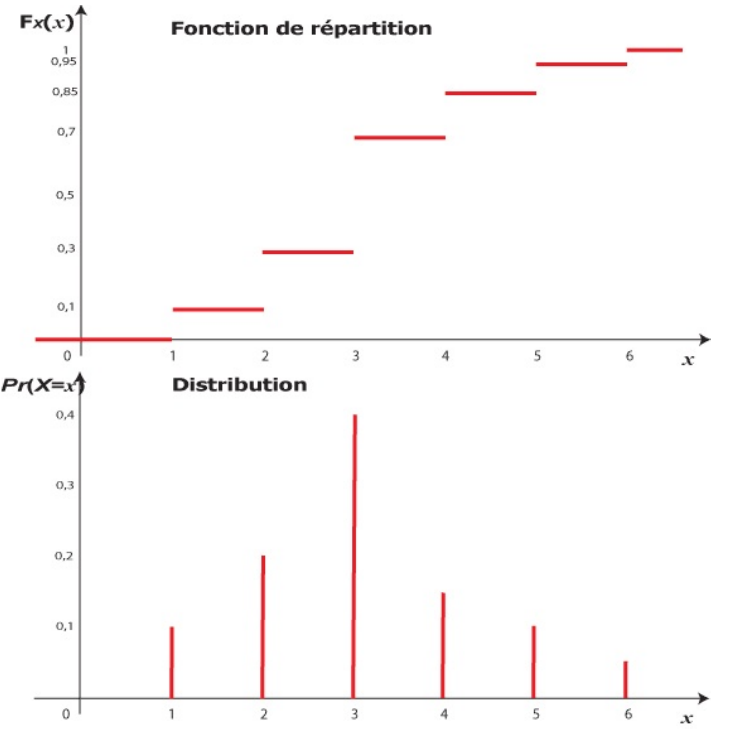
\includegraphics[width=8cm]{content/figureremarque1.PNG}
\end{figure}
%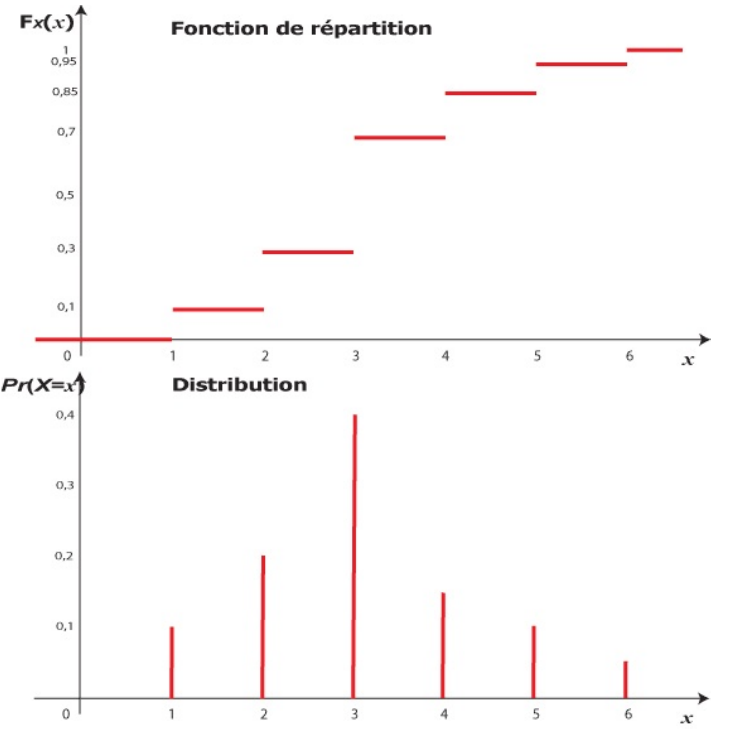
\includegraphics{content/figureremarque1.PNG}
\end{remark}






































\iffalse
\section{Loi d’une variable aléatoire réelle - Fonction de répartition}\label{chap:1}

% This is a comment
Ici, nous discutons des concepts nécessaires pour tirer des conclusions statistiques à partir d'un échantillon de
données sur une population d'intérêt. Par exemple, supposons que nous connaissions le salaire de départ d'un
échantillon de 100 étudiants diplômés en droit. Nous pouvons utiliser ces connaissances pour tirer des conclusions
sur le salaire prévu pour la population de tous les étudiants diplômés en droit. De même, si un médicament nouvellement
développé est administré à un échantillon de patients tuberculeux sélectionnés, alors certains patients peuvent montrer
une amélioration et d'autres non, mais nous nous intéressons aux conséquences pour l'ensemble de la population de
patients. Dans la suite de ce chapitre, nous décrivons les concepts théoriques nécessaires pour tirer de telles
conclusions. Ils constituent la base des tests statistiques et de l'inférence.


\subsection{Variables aléatoires}
Les variables aléatoires nous aident à voir les données collectées comme le résultat d'une expérience aléatoire.
Considérez l'expérience simple de lancer une pièce. Si une pièce est lancée, alors on peut observer soit «face» (F)
ou «pile» (P). L'apparition de «face» ou de «pile» est aléatoire, et le résultat exact ne sera connu qu'après avoir
lancé la pièce. Nous pouvons lancer la pièce plusieurs fois et obtenir une séquence de sorties. Par exemple, si une
pièce est lancée sept fois, puis l'un des résultats peut être F, F, P, F, P, P, P. Ce résultat est la conséquence
d'une expérience aléatoire, et il peut être utile de distiller la séquence des résultats en nombres significatifs.
Une option consiste à les résumer par une variable $X$, qui prend les valeurs $x_1 = 1$ (pour pile) et $x_2 = 0$
(pour face). Cela peut être décrit dans le cadre d'une expérience aléatoire où $\Omega= \{\omega_1, \omega_2\}$ avec les événements
$A_1 = \{\omega_1\} = 1 = \text{pile}$ et $A_2 = \{\omega_2\} = 0 = \text{face}$.\\

La variable aléatoire $X$ est désormais associée à des nombres réels et, par conséquent, elle décrit le résultat possible
de toute expérience de lancer de pièces. Les résultats observés F, F, P, F, P, P, P se rapportent à un échantillon
spécifique, une réalisation unique de cette expérience. On peut écrire $X(\omega_1) = 1$ et $X(\omega_2) = 0$ avec
$\omega_1, \omega_2 \in \Omega$
et $1,0 \in \mathcal{R}$ où $\mathcal{R}$ est l'ensemble des nombres réels. Nous savons que dans toute expérience de lancer de pièces, la
probabilité que face soit observée est $P (X (\omega_1) = 1) = 0,5$ et que pile observée est
$P (X (\omega_2) = 0) = 0,5$. Nous pouvons donc considérer $X$ comme une variable aléatoire qui recueille les
résultats possibles d'une expérience aléatoire et capture l'incertitude qui leur est associée.

\begin{table}[h!]
    \centering
    \caption{Exemples de variables aléatoires}
    \begin{tabular}{||c | c | c ||}
        \hline
        $X$ & Événement  & Réalisations de $X$\\ [0.5ex]
        \hline\hline
        Lancer d'un dé & $A_i$: nombre $i$ ($i = 1, 2,\dots, 6$) & $x = i$ \\\hline
        Durée de d'une TV & $A_i$: temps de survie est $i$ mois $(i = 1, 2, \dots)$ & $x = i$  \\\hline
        Roulette (Jeu de hasard) &\makecell{  $A_1$: rouge\\ $A_2$: noir\\\ $A_3$: vert (zéro)} &\makecell{ $x_1=1$\\$x_2=2$\\ $x_3=0$} \\ [1ex]
        %info & \makecell{ line1 \\\hline line2 }  &  blubb&\\
        \hline
    \end{tabular}

    \label{table:1}
\end{table}

\theoremstyle{definition}
\begin{definition}{}
Soit $\omega$ représente l'espace échantillon d'une expérience aléatoire, et soit $\mathcal{R}$ l'ensemble des nombres
réels. Une variable aléatoire est une fonction $X$ qui attribue à chaque élément $\omega \in \Omega$ un et un seul
nombre $X (\omega) = x, x \in \mathcal{R}$, c'est-à-dire.
\begin{equation}
    X : \Omega \to \mathcal{R}
\end{equation}
\end{definition}

\begin{example}
    Les caractéristiques d'une expérience de jet de dé, d'un jeu de roulette ou de la durée de vie d'un téléviseur
    peuvent toutes être décrites par une variable aléatoire, voir Tableau \ref{table:1}. Les événements impliquent un
    caractère aléatoire, et si nous avons des connaissances sur le processus aléatoire, nous pouvons attribuer des
    probabilités $P (X = x_i)$ à chaque événement, par ex. lors du lancer d'un dé, la probabilité d'obtenir
    un «$1$» est $P (X = 1) = 1/6$ et la probabilité d'obtenir un «$2$» est $P (X = 2) = 1/6$.
\end{example}
Plus généralement, on peut dire qu'il est obligatoire de connaître $ P (X \in A) $ pour tous les $ A $ possibles qui sont
des sous-ensembles de $ \ mathcal {R} $. Si nous choisissons $ A = (-\infty, x], x ∈ \ mathcal {R} $, nous avons
$$ P(X\in A) = P(X\in (-\infty,x])=P(-\infty<X\leq x)=P(x\leq x). $$
Cette considération donne lieu à la définition de la Fonction de répartition.

\subsection{Fonction de répartition}
\theoremstyle{definition}
\begin{definition}{}\label{def:foncrep}

La fonction de répartition (\textbf{cumulative distribution function}) d'une variable aléatoire X est définie comme

\begin{equation}
    F(x) = P(X\leq x).
\end{equation}
\end{definition}
Nous pouvons voir que la fonction de répartition est utile pour obtenir les probabilités liées à l'occurrence d'événements
aléatoires. Notons que la Fonction de répartition empirique\footnote{La fonction de répartition empirique $ F (x) $ est
définie comme:
\begin{equation}
    F(x) = \sum_{a_j\leq x}f(a_j)
\end{equation}
avec $f_j =n_j/n$, $n$ le nombre d'observation.\\ Cette définition implique que F (x) est une fonction monotone non
décroissante, $0\leq F(x)\leq1$, $\lim_{x \to-\infty}F(x) = 0$, $\lim_{x \to+\infty}F(x) = 1$, et F(x) est continue à
droite.} et la Fonction de répartition sont étroitement liées et ont donc une définition et des règles de calcul
similaires.\\

La Définition \ref{def:foncrep} applique les propriétés suivantes de la fonction de répartition:
\begin{itemize}
\item $F(x)$ est une fonction monotone non décroissante (si $x_1\leq x_2$, alors $F(x_1)\leq F(x_2)$),
\item $\lim_{x\to-\infty}F(x)=0$ (la limite inf de $F$ est $0$),
\item $\lim_{x\to+\infty}F(x)=1$ (la limite sup de $F$ est $1$),
\item $F(x)$ est continue à droite, et
\item $0\leq F(x)\leq1$ pour tout $x\in\mathcal{R}$.
\end{itemize}
Une autre notation pour $F(x)=P(X\leq x)$ est $F_{X}(x)$, mais on utilisera $F(x)$

\subsubsection{La fonction de répartition des variables aléatoires continues}
Avant de donner quelques exemples sur la signification et l'interprétation de la fonction de répartition, nous devons
d'abord considérer quelques définitions et théorèmes.

\theoremstyle{definition}
\begin{definition}{}\label{def:vacont}
Une variable aléatoire $ X $ est dite \textbf{continue} s'il y a une fonction
$ f (x) $ tel que pour tout $ x \in \mathcal {R} $
\begin{equation}
F(x) = \int_{-\infty}^{x}f(t)d(t)
\end{equation}
existe. $F(x)$ est la fonction de répartition de $X$, et $f(x)$  est la densité de probabilité de $x$ et
$\frac{d}{dx}F(x)=f(x)$ pour tous les $x$ qui sont des points de continuité de $f$.
\end{definition}
\theoremstyle{theorem}
\begin{theorem}{}\label{thm:1.1}
Pour qu'une fonction $ f (x) $ soit une fonction de densité de probabilité de $ X $, elle doit satisfaire aux
conditions suivantes:
\begin{enumerate}
\item $f(x)\geq0$ pour tout $x\in\mathcal{R}$
\item $\int_{-\infty}^{+\infty}f(x)dx=1$.
\end{enumerate}
\end{theorem}

\theoremstyle{theorem}
\begin{theorem}{}\label{thm:1.2}
Soit $ X $ une variable aléatoire avec une fonction de répartition $ F (x) $. Si $ x_1 <x_2 $,
où $ x_1 $ et $ x_2 $ sont des constantes connues,
$ P (x_1 \leq X \leq x_2) = F (x_2) - F (x_1) = \int_ {x_1} ^ {x_2} f (x) dx $.
\end{theorem}

\theoremstyle{theorem}
\begin{theorem}\label{thm:1.3}
La probabilité qu'une variable aléatoire continue prenne une valeur particulière $ x_0 $ est nulle:
\begin{equation}
P(X=x_0)=0.
\end{equation}
\end{theorem}
\begin{pruf}
Considérons un intervalle $(x_0-\delta,x_0]$ avec $\delta\geq0$. Il découle du Théorème \ref{thm:1.2} que
$P(x_0-\delta<X\leq x_0)=F(x_0)-F(x_0-\delta)$ et donc

\begin{align*}
P(X=x_0) & = \lim_{\delta\to0}P(x_0 -\delta<X\leq x_0)\\&= \lim_{\delta\to0}[F(x_0) - F(x_0 -\delta)]\\&= F(x_0) - F(x_0) =0.
\end{align*}
\end{pruf}

\begin{example}\label{exemple:1}
Prenons la variable aléatoire continue «temps d'attente pour le train». Supposons qu'un train arrive toutes les 20 min.
Par conséquent, le temps d'attente d'une personne particulière est aléatoire et peut être n'importe quel temps contenu
dans l'intervalle $ [0, 20] $. Nous pouvons commencer à décrire la fonction de densité de probabilité requise comme

$$f(n) = \begin{cases} k, & \mbox{pour   } 0\leq x\leq20 \\ 0, & \mbox{ailleurs } \end{cases}$$

où $k$ est une constante inconnue. Maintenant, en utilisant la condition (2) du Théorème \ref{thm:1.1}, on a
$$1=\int_0^{20}f(x)dx=[kx]_{0}^{20}=20k$$
qui doit être remplie. Cela donne $ k = 1/20 $ qui est toujours supérieur à 0, et par conséquent, la condition (1)
du Théorème \ref{thm:1.1} est également remplie. Il s'ensuit que

$$f(n) = \begin{cases} \frac{1}{20}, & \mbox{pour   } 0\leq x\leq20 \\ 0, & \mbox{ailleurs } \end{cases}$$

est la fonction de densité de probabilité décrivant le temps d'attente pour le train. Nous pouvons maintenant utiliser
Définition \ref{def:vacont} pour déterminer la fonction de répartition:
$$F(x)=\int_{0}^{x}f(t)dt=\int_{0}^{x}\frac{1}{20}dt=\frac{1}{20}[t]_{0}^{x}=\frac{1}{20}x.$$
Supposons que nous souhaitons calculer la probabilité d'un temps d'attente compris entre 15 $ et 20 $ min.
Cela peut être calculé en utilisant le Théorème \ref{thm:1.2}:
$$P(15\leq X\leq20)=F(20)-F(15)=\frac{20}{20}-\frac{15}{20}=0.25.$$
Nous pouvons également obtenir cette probabilité à partir du graphique de la fonction de répartition, voir Fig. \ref{fig:exemple1}
où la densité de probabilité et la fonction de répartition de cet exemple sont illustrées.\\

La définition d'une fonction, par exemple la fonction de répartition, est simple dans R: on peut utiliser
la commande \textit{function} suivie de la spécification des variables que la fonction évalue entre parenthèses
(par exemple $ x $) et la fonction elle-même entre accolades (par exemple $ x / 20 $ ). Les fonctions peuvent être
tracées à l'aide de la commande \textit{curve}:

\begin{verbatim}
cdf <- function(x){1/20*x}
curve(cdf,from=0,to=20)
\end{verbatim}


\begin{figure}%
\centering
\subfloat[Fonction de densité de probabilité]{{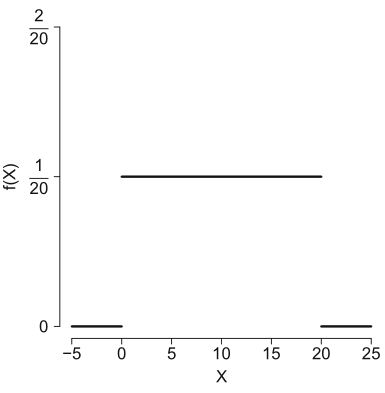
\includegraphics[width=5cm]{content/pdf.PNG} }}%
\qquad
\subfloat[Fonction de répartition]{{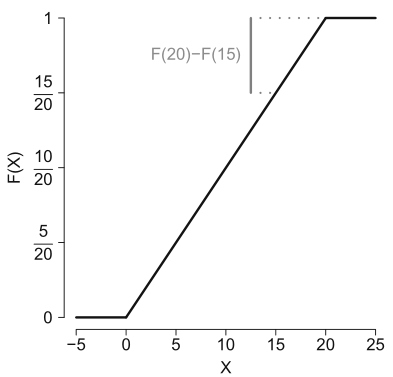
\includegraphics[width=5cm]{content/cdf.PNG} }}%
\caption{Fonction de densité de probabilité et fonction de répartition pour le temps d'attente dans l'exemple \ref{exemple:1}}%
\label{fig:exemple1}%
\end{figure}
\end{example}
\subsubsection{La fonction de répartition des variables aléatoires discrètes}

\theoremstyle{definition}
\begin{definition}
Une variable aléatoire $X$ est définie comme étant \textbf{discrète} si son espace de probabilité est fini ou dénombrable,
c'est-à-dire si elle ne prend qu'un nombre fini ou dénombrable de valeurs. Notez qu'un ensemble $V$ est censé
être \textbf{dénombrable}, si ses éléments peuvent être listés, c'est-à-dire qu'il existe une bijection entre $V$
et les entiers positifs.
\end{definition}

\begin{example}\label{exemple:2}
Prenons l'exemple du lancement d'une pièce où chaque essai donne lieu à face (F) ou à pile (P), chacune se produisant
avec la même probabilité $0,5$. Lorsque la pièce est lancée plusieurs fois, nous pouvons observer des séquences telles
que F, P, F, F, P, F, F, P et P, \dots. L'espace d'échantillon est $\Omega = \{F, P\}$. Soit la variable aléatoire $X$ le
nombre d'essais requis pour obtenir la troisième tête, puis $X = 4$ pour la séquence donnée ci-dessus.
Clairement, l'espace de $X$ est l'ensemble $(3,4,5, \dots)$. Nous pouvons voir que $X$ est une variable aléatoire
discrète car son espace est fini et peut être compté. Nous pouvons également attribuer certaines probabilités à
chacune de ces valeurs, par exemple $P (X = 3) = p_1$ et $P (X = 4) = p_2$.
\end{example}

\theoremstyle{definition}
\begin{definition}
Soit $X$ une variable aléatoire discrète qui prend $k$ valeurs différentes.
La \textbf{fonction de masse} de probabilité (probability mass function) de $X$ est donnée par
\begin{equation}\label{eq:foncmass}
f(X) = P(X = x_i)=p_i \text{ pour tout } i=1,2,\dots,k.
\end{equation}
Il est nécessaire que les probabilités $p_i$ remplissent les conditions suivantes:
\begin{enumerate}
\item $0\leq p_i\leq1$,
\item $\sum_{i=1}^{k}p_i=1$.
\end{enumerate}
\end{definition}

\theoremstyle{definition}
\begin{definition}
Étant donné (\ref{eq:foncmass}), nous pouvons écrire la fonction de répartition d'une variable aléatoire discrète comme
\begin{equation}\label{eq:frvd}
F(x)=\sum_{i=1}^{k} \mathds{1}_{\{x_i \leq x\}}p_i,
\end{equation}
où $\mathds{1}$ est une fonction indicatrice définie comme
$$\mathds{1}_{\{x_i \leq x\}} = \begin{cases} 1, & \mbox{si   } x_i\leq x\\ 0, & \mbox{ailleurs } \end{cases}$$
\end{definition}

La fonction de répartition d'une variable discrète est toujours une \textbf{fonction en escalier}.\\

Nous pouvons facilement calculer différents types de probabilités pour des variables aléatoires discrètes en utilisant
la fonction de répartition. Soit $ a $ et $ b $ des constantes connues, alors
\begin{align}\label{eq:freqs}
P(X\leq a) & = F(a),\label{sub-eq-1:8}\\P(X<a) &= P(X\leq a)-P(X=a)=F(a)-P(X=a),\\P(X>a) &= 1-P(X\leq a)=1-F(a),\\
P(X\geq a) &=1-P(X<a)=1-F(a)+P(X=a),\\ \nonumber P(a\leq X\leq b) &= P(X\leq b) - P(X<a)\\ &=F(b)-F(a)+P(X=a),\\
P(a<X\leq b) &= F(b)-F(a),\\P(a<X<b) &= F(b)-F(a)-P(X=b),\label{sub-eq-1:14}\\P(a\leq X<b)&=F(b)-F(a)-P(X=b)+P(X=a).\label{sub-eq-1:1}
\end{align}
\begin{remark}
Les équations (\ref{eq:frvd})-(\ref{sub-eq-1:1}) peuvent également être utilisées pour les variables continues, mais dans ce cas,
$P (X = a) = P (X = b) = 0$ (voir le Théorème \ref{thm:1.3}), et donc les équations (\ref{eq:frvd})-(\ref{sub-eq-1:1}) peut être modifié en conséquence.
\end{remark}

\begin{example}\label{exemple:4}
Considérons l'expérience de lancer un dé. Il y a six résultats possibles. Si nous définissons la variable aléatoire $X$
comme le nombre de points observés sur la surface supérieure du dé, alors les six résultats possibles peuvent être
décrits comme $x_1 = 1, x_2 = 2,\dots, x_6 = 6$. Les probabilités respectives sont $P (X = x_i) = 1/6$; $i = 1,2, ..., 6$.
La fonction de masse et la fonction de répartition sont donc définies comme suit:

\begin{equation}
f(n) = \begin{cases} 1/6 & \mbox{si   } x=1 \\1/6 & \mbox{si   } x=2 \\1/6 & \mbox{si   } x=3 \\1/6 & \mbox{si   } x=4 \\1/6 & \mbox{si   } x=5 \\1/6 & \mbox{si   } x=6 \\ 0 & \mbox{ailleurs } \end{cases}
\quad\mathrm{   }\quad
f(n) = \begin{cases} 0 & \mbox{si   } -\infty<x<1 \\1/6 & \mbox{si   } 1\leq x<2 \\2/6 & \mbox{si   } 2\leq x<3 \\3/6 & \mbox{si   } 3\leq x<4 \\4/6 & \mbox{si   } 4\leq x<5 \\5/6 & \mbox{si   } 5\leq x<6 \\ 1 & \mbox{si } 6\leq x<\infty \end{cases}
\end{equation}

\begin{figure}%
\centering
\subfloat[Fonction de densité de probabilité]{{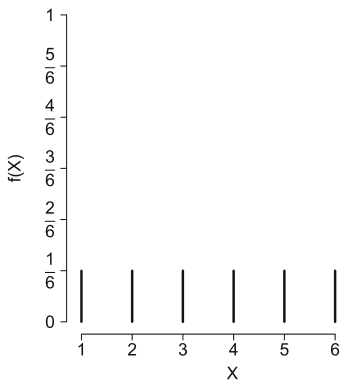
\includegraphics[width=5cm]{content/pdfdiscret.PNG} }}%
\qquad
\subfloat[Fonction de répartition]{{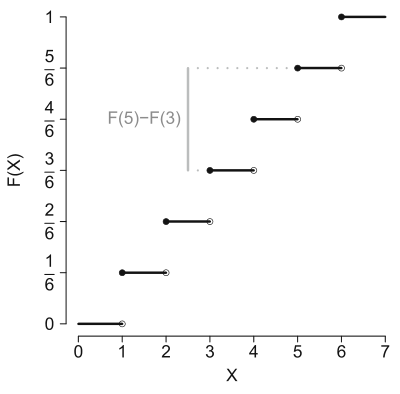
\includegraphics[width=5cm]{content/cdfdiscret.PNG} }}%
\caption{Fonction de densité de probabilité et fonction de répartition pour
le lancer d'un dé dans l'exemple \ref{exemple:4}. «•» se rapporte à une valeur incluse et «$\circ$» à une valeur exclue}%
\label{fig:exemple4}%
\end{figure}

\end{example}

Nous pouvons utiliser la fonction de répartition pour calculer toute probabilité souhaitée, par exemple
$P (X ≤ 5) = F (5) = 5/6$. Ceci est montré sur la figure \ref{fig:exemple4}b où pour $X = 5$, nous obtenons
$F (5) = 5/6$ lors de l'évaluation sur l'axe des $y$. De même, $P (3 <X ≤ 5) = F (5) - F (3) = (5/6) - (3/6) = 2/6$
peut être interprété comme la différence de $F (5)$ et $F ( 3) $ sur l'axe des $y$.





%Here I am talking about a great article \cite{great_article}. And there is also a great conference proceedings \cite{great_proceedings}.

\subsection{Figures}

Here is an example of a figure environment :

\begin{center}
    \begin{figure}[ht!]
        \centering
        
        
\includegraphics[width=5cm, keepaspectratio]{imports/2000.png}
        
        \caption{This is a figure description}
    \end{figure}
\end{center}

\subsection{Item lists}

This is a list of items :

\begin{itemize}
    \item Item 1
    \item Item 2
    \item Item 3
\end{itemize}

\subsection{Footnotes}

This is a footnote \footnote{footnote content}.

\subsection{Tabular}


\begin{center}
    \begin{tabular}{|l|c|r|} % left - center - right
        \hline
        \rowcolor{white!75!black} \textbf{Column 1} & \textbf{Column 2} & \textbf{Column 3} \\
        \hline
        Left aligned lalalalala & centered & Right aligned lalalalala\\
        \hline
         & & \\
        \hline
    \end{tabular}
\end{center}
\fi
\newpage

\section{Loi d’une variable aléatoire à densité}

\subsection{Variable aléatoire à densité}

\theoremstyle{definition}
\begin{definition}

    \begin{enumerate}
        \item Soit $X$ une variable aléatoire. On dit que $X$ \textbf{a une loi de densité $f$}
        et que $P_{\textbf{X}}$  \textbf{a pour densité} $f$, si pour tout réel $x$,
\textcolor{blue}{$$F_{\textbf{X}}(x)=\mathbb{P}_{\textbf{X}}(]-\infty,x])=\mathbb{P}(X\leq x)=\int_{-\infty}^{x}f(y)fy.$$}
       Dans ce cas $$\mathbb{P}(X=x)=0, \mbox{   } \forall x\in \mathbb{R}.$$
        \item  Une fonction réelle $f$ sur $\mathbb{R}$ est appelée une \textbf{densité de probabilité},
ou simplement une “densité”, si elle est \textcolor{blue}{positive, intégrable}, et vérifie
\textcolor{blue}{$$\int_{_\infty}^{+\infty}f(x)dx=1.$$}
    \end{enumerate}
\end{definition}

\theoremstyle{remarkfonda}
\begin{remarkfonda}
Si $f$ est une densité de probabilité, la fonction $F$ définie par $$F(x)=\int_{-\infty}^{x}f(y)dy$$
est une fonction qui vérifie les propriétés (\ref{prop:prop1.1}), (\ref{prop:prop1.2}), (\ref{prop:prop1.3}).
Elle permet donc de définir une unique probabilité $\mu$ sur \mathbb{R}, telle que $$\mu(]-\infty,x])=\int_{-\infty}^{x}f(y)dy.$$
si $\mu$ est la loi de $X$, alors $\mathbb{P}(X\leq x)=\int_{-\infty}^{x}f(y)dy.$

\begin{figure}[h]
\centering
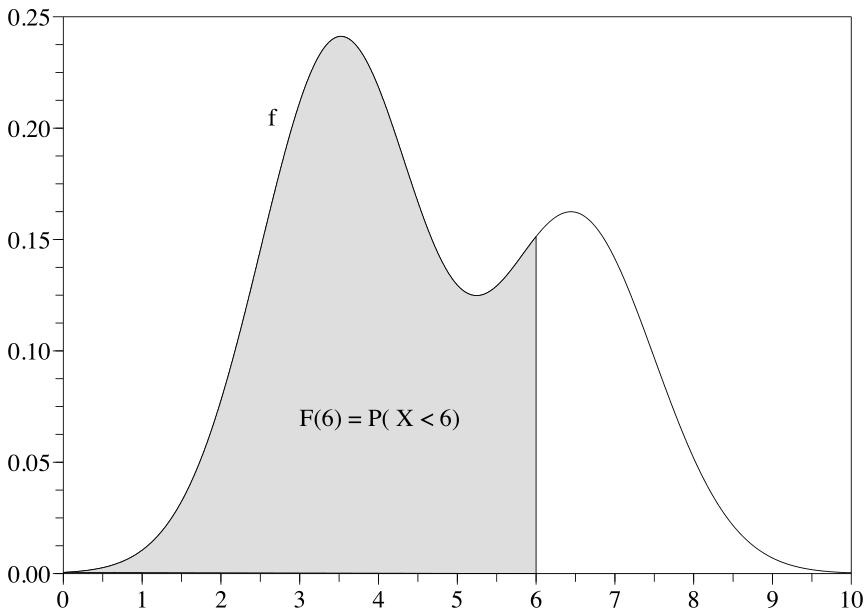
\includegraphics[width=5.5cm]{content/densite.PNG}
\caption{Graphe de la densité $f$.}
\end{figure}
\end{remarkfonda}

\theoremstyle{proposition}
\begin{proposition}
\begin{enumerate}
\item Soit $X$ de loi de densité $f$. La fonction $F_X$ est dérivable en tout point
$x$ où $f$ est continue, et \textcolor{blue}{$$F'_{X}(x)=f(x).$$}
\item  Si $F_X$ est dérivable en tout point, alors $X$ a une loi de densité \textcolor{blue}{$$f=F'_{X}.$$}
\end{enumerate}

\end{proposition}

\begin{pruf}
Dérivée d’une intégrale fonction de sa borne supérieure.
\end{pruf}

\theoremstyle{interpretation*}
\begin{interpretation*}
si $\Delta x$  est un “petit” accroissement de la quantité $x$, on
a (si du moins $f$ est continue en $x$):
$$f(x)\sim\frac{F_X(x+\Delta x)-F_X(x)}{\Delta x}=\frac{\mathbb{P}_X([x,x+\Delta x])}{\Delta x}.$$
\begin{figure}[h]
\centering
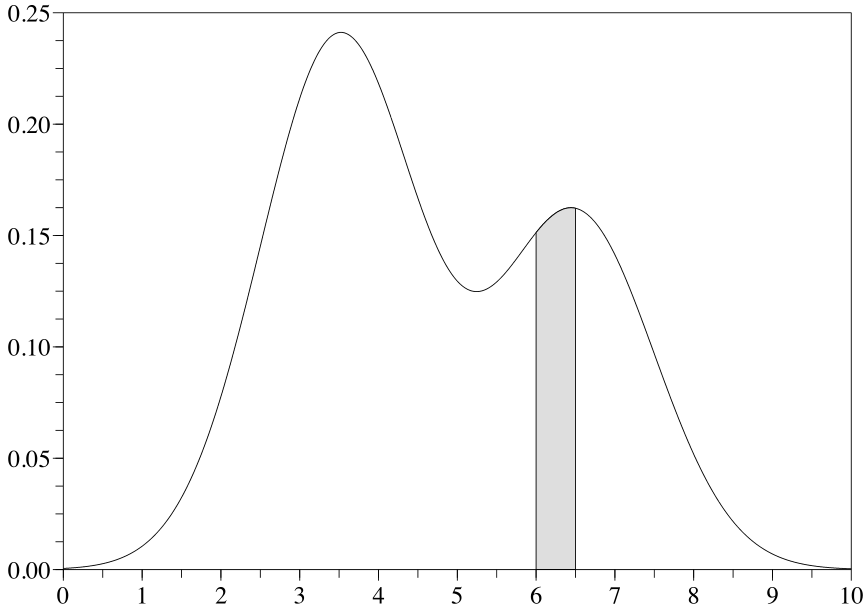
\includegraphics[width=8cm]{content/interpretation1.PNG}
\caption{$f(6)\sim\frac{(F_X(6.5)-F_X(6))}{0.5}$.}
\end{figure}

\end{interpretation*}

\subsection{Lois usuelles et simulation}
\subsubsection{Variable aléatoire uniforme}
\textbullet \textcolor{blue}{Variable aléatoire uniforme sur $[a,b]$, $a < b$}: $X(\Omega)=[a,b]$, et
\textcolor{red}{$$f(x) = \begin{cases} \frac{1}{b-a} & \mbox{si   } a\leq x\leq b\\
                                        0 & \mbox{sinon } .\end{cases}$$}
Autant de chances de tomber au voisinage de chaque point de $[a,b]$.

\begin{example}
Horaires navette Massy-Ecole Polytechnique : 8h12, 8h20,
8h26, 8h32.
\begin{itemize}
\item L’arrivée du RER suit une variable uniforme sur [8h15,8h30].
\item Probabilité d’attendre la navette moins de 3 minutes?
\item Probabilité d’attendre plus de 5 minutes?
\end{itemize}
\end{example}

\subsubsection{Simulation d’une variable aléatoire}
\begin{itemize}
\item \textbf{But: générer les valeurs d’une variable aléatoire X de
fonction de répartition F donnée}.
\item Cas le plus simple:\textcolor{blue}{ simuler les valeurs d’une variable aléatoire $U$
de loi uniforme sur $[0,1]$}.
\item On utilise un générateur de nombres pseudo-aléatoires: fonction
“RANDOM” de l’ordinateur.
\item Pour simuler $X$, on peut souvent se ramener à la simulation de $U$$,\\
\textbf{ en utilisant une inversion de la fonction de répartition de } $X$$.
\end{itemize}

\theoremstyle{theorem}
\begin{theorem}
Soit $F$ une fonction vérifiant les propriétés (\ref{prop:prop1.1}), (\ref{prop:prop1.2}), (\ref{prop:prop1.3}).
Soit $F^{−1} : ]0,1[\rightarrow\mathbb{R}$, l’inverse généralisée de $F$:
\textcolor{blue}{$$F^1(u)=\min\{x\in\mathbb{R}, F(x)\geq u\},$$}
alors $X = F^{−1}(U)$ est une variable aléatoire de loi $\mathbb{P}_{\textbf{X}}$ , où $\mathbb{P}_{\textbf{X}$ a pour
fonction de répartition $F$.
\end{theorem}

\begin{pruf}
$$\mathbb{P}(X\leq x)=\mathbb{P}(F^{-1}(U)\leq x)=\mathbb{P}(U\leq F(x))=F(x).$$
\end{pruf}

\begin{conclusion}
Pour simuler $X$, on simule $U$ en utilisant $rand$ et on
calcule son image par $F^{-1}$.
\end{conclusion}

\begin{example}
\textcolor{blue}{ $X$ variable aléatoire de Bernoulli de paramètre $p$}.
\begin{itemize}
\item Si $U\in[0,1-p[$, on pose $X=0$,
\item Si $U\in[1-p,1]$, on pose $X=1$.
\end{itemize}
\end{example}

\subsubsection{Variable aléatoire exponentielle}
\theoremstyle{definition}
\begin{definition}
X \textbf{suit la loi exponentielle de paramètre} $\lambda>0$ : $X(\Omega)=\mathbb{R}_{+}$ et $\mathbb{P}_X$ admet la loi
de densité \textcolor{blue}{
$$f(x) = \begin{cases} 0 & \mbox{si   } x<0\\
\lambda e^{-\lambda x} & \mbox{sinon } .\end{cases}$$
}
On la note \textcolor{blue}{$\mathcal{E}(\lambda)}.$
\end{definition}

Modélisation d’une durée de vie ou d’un temps d’attente entre
événements spécifiques:
\begin{itemize}
\item durée de vie d’une bactérie
\item durée d’une conversation téléphonique
\item temps entre deux tremblements de terre.
\end{itemize}

\subsubsection{Loi exponentielle sans mémoire}
$X:\Omega\rightarrow\mathbb{R}_{+}.$\\
\textbf{Propriété de non-vieillissement}:$$\mathbb{P}(X>t+s|X>t)=\mathbb{P}(X>s)=e^{-\lambda s}.$$
\begin{example}
hypothèse naturelle pour modéliser des durées de vie d’atomes
radioactifs.
\end{example}

\vskip 1cm

\textbf{Propriété caractéristique}: si $t\rightarrow\rho(t)=\mathb{P}(X>t)$ verifie
\textcolor{red}{$$\rho(t+s)=\rho(t)\rho(s)$$}
on a (en dérivant en $s$, avec $s = 0$),
$$\rho'(t)=-\rho(t)\lambda \quad\mathrm{  avec  }\quad \lambda=-\rho'(0)\geq0.$$
Ainsi \textcolor{blue}{$\rho(t)=e^{-\lambda t}$ et $f(t)=\lamda e^{-\lambda t}$ (Loi exponentielle)}. ($\rho(0)=1$.)
\vskip 1cm
\textbf{Simulation d’une v.a. de loi} $\mathcal{E}(\lambda), \lambda>0$:
\textcolor{blue}{$$F(x)=\int_{0}^{x}\lambda e^{-\lambda t}dt=1-e^{-\lambda x},\quad\mathrm{  }\quad\forall x\geq0.$$}
Ainsi, si $u\in[0,1[$,$$F^{-1}(u)=-(1/\lambda)\log(1-u).$$
On simulera donc une loi uniforme $U$ et on posera \textcolor{red}{$$X=-\frac{1}{\lambda}\log U.$$}
$X$ est une variable aléatoire de loi $\mathcal{E}(\lambda)$.\\
En effet, les variables aléatoires $U$ et $1-U$ ont même loi.

\subsubsection{Lois Gamma}
\theoremstyle{definition}
\begin{definition}
$X$ \textbf{suit la loi gamma de paramètres} $\beta,\alpha>0$ si $X(\Omega)=\mathbb{R}_{+}$ et $\mathbb{P}_X$
admet la loi de densité
\textcolor{blue}{$$f(x) = \begin{cases} 0 & \mbox{si   } x<0\\ \frac{1}{\Gamma(\alpha)}\beta^{\alpha}x^{\alpha-1}e^{-\beta x} & \mbox{sinon}.\end{cases}$$}
\end{definition}

\begin{figure}[h]
\centering
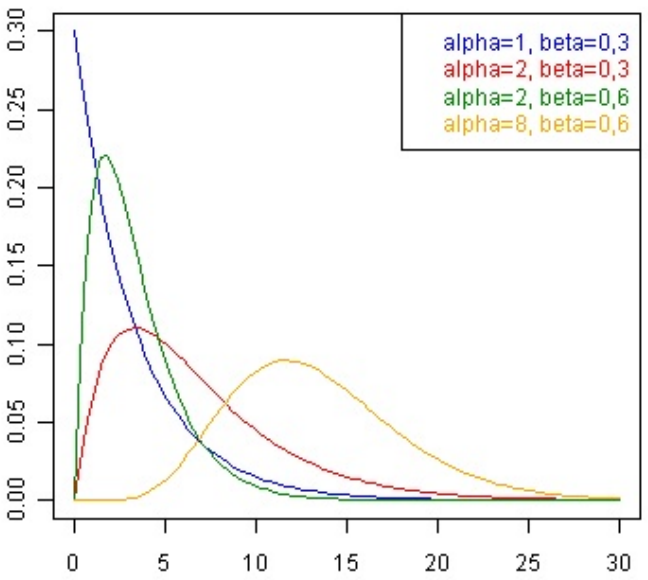
\includegraphics[width=8cm]{content/gamma.PNG}
\caption{Densités Gamma.}
\end{figure}

\subsubsection{Variable aléatoire normale (variable gaussienne)}

\theoremstyle{definition}
\begin{definition}
On appelle \textbf{variable aléatoire normale centrée réduite} une variable
aléatoire $X$ de loi de densité \textcolor{blue}{$$f(x)=\frac{1}{\sqrt{2\pi}}e^{-x^2/2}.$$}
\end{definition}

\begin{remark}
$$I=\int_{-\infty}^{+\infty}f(x)dx=1.$$
En effet \textcolor{blue}{
\begin{align*}
I^2 &=\int_{\mathbb{R}}\int_{\mathbb{R}}f(x)f(y)dxdy=\frac{1}{2\pi}\int\int e^{-\frac{(x^2+y^2)}{2}}dxdy\\
    &=\int_{0}^{2\pi}d\theta\int_{0}^{\infty}\frac{1}{2\pi}e^{-\rho^2/2}\rho d\rho=1.\text{ (passage en polaire)}
\end{align*}
}
$f$ \textbf{n’a pas de primitive évidente}: tables numériques.
\end{remark}

Pour $m\in\mathbb{R},\sigma>0$, \textbf{une variable normale $Y$ de loi $\mathcal{N}(m,\sigma)$ a pour densité}
\textcolor{blue}{$$f(y)=\frac{1}{\sqrt{2\pi\sigma^2}}\exp(-\frac{(y-m)^2}{2\sigma^2}).$$}
\textbf{Distribution normale}:
\begin{itemize}
\item taille d’un individu choisi au hasard
\item composantes de la vitesse d’une molécule de gaz
\item erreur de mesure d’une quantité physique.

\end{itemize}
taille d’un individu choisi au hasard
composantes de la vitesse d’une molécule de gaz
erreur de mesure d’une quantité physique.

\textcolor{blue}{Approximation de toute somme de variables aléatoires indépendantes
et de même loi: \textbf{théorème de la limite centrale}.}


\begin{figure}[h]
\centering
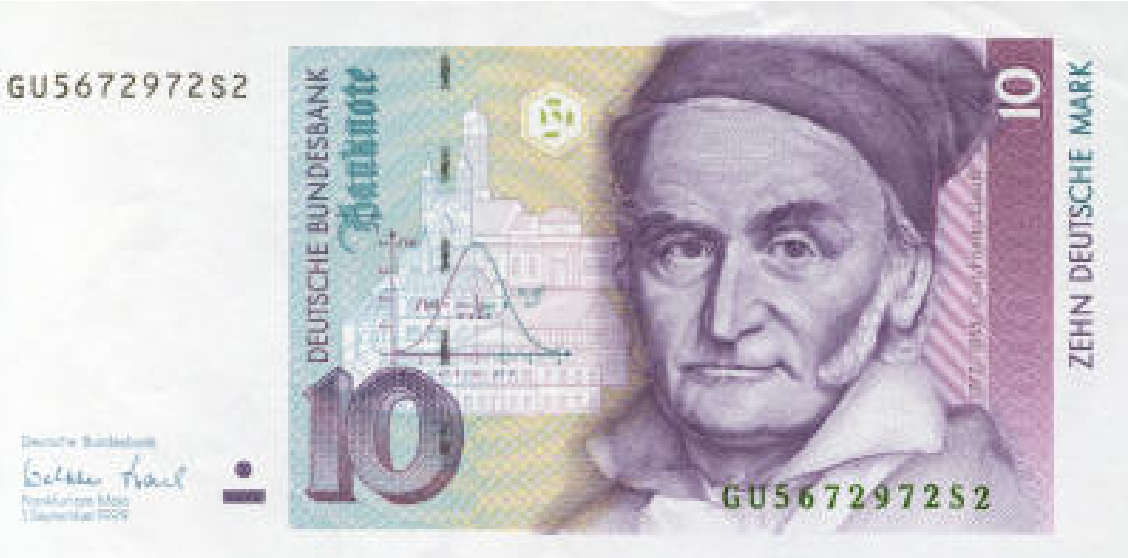
\includegraphics[width=8cm]{content/money.PNG}

\end{figure}

\section{Simuler des variables aléatoires}

\textbf{But} :
générer une $X$ variable aléatoire à partir d’une
variable aléatoire uniforme $U \sim \mathcal{U}([0,1])$.
%%%%%%%%%%%%%%%%%%%%%%%%%%%%%%%%%%%%%%%%%%%%%%%%%%%%%%%%%%%%%%%%%%%%%%%%%%%%%%%%
%%%%%%%%%%%%%%%%%%%%%%%%%%%%%%%%%%%%%%%%%%%%%%%%%%%%%%%%%%%%%%%%%%%%%%%%%%%%%%%%
%%%%%%%%%%%%%%%%%%%%%%%%%  partie de lecheguer  %%%%%%%%%%%%%%%%%%%%%%%%%%%%%%%%
%%%%%%%%%%%%%%%%%%%%%%%%%%%%%%%% DEBUT %%%%%%%%%%%%%%%%%%%%%%%%%%%%%%%%%%%%%%%%%
%%%%%%%%%%%%%%%%%%%%%%%%%%%%%%%%%%%%%%%%%%%%%%%%%%%%%%%%%%%%%%%%%%%%%%%%%%%%%%%%
\subsection{Simuler le hasard avec un ordinateur}

\textcolor{gray}{De très nombreuses applications: \\}
Simulations de phénomènes physiques, méthodes de
Monte-Carlo pour le calcul d'intégrales, étude de tests
statistiques, simulation de fonctionnement de réseaux,
cryptographie, imagerie, algorithmes probabilistes, etc. \\
\vspace{0.5cm}

Pourquoi le terme \textcolor{blue}{SIMULER}? \\
Parce qu'un ordinateur exécute un algorithme, c'est-à-dire une suite d'opérations parfaitement déterminées.\\
L'idée est de produire une suite de nombres suffisamment
imprévisibles qui « imite » une suite $(U_{n})_{n \geq 1}$ de variables aléatoires indépendantes uniformes dans l'intervalle [0,1[.\\

\vspace{1cm}

\begin{Large}
\colorbox{gray!20}{\textcolor{blue}{Fonction " \textbf{random} " des langages de programmation
courants}}
\end{Large}

Elle est basée sur la suite de nombres $(X_{n})_{n \geq 1}$ vérifiant une relation de récurrence
\[ X_{n+1} = (a X_{n}+ c) \mod M \]
On prend
\[ U_{n} = \dfrac{X_{n}}{M} \in [0,1[ \]

Exemple de \textit{Scilab} \emph{(https://www.scilab.org/fr)} : \\
\[ M = 2^{31} ; \hspace{2mm} a= 843 314 861; \hspace{2mm} c= 453 816 693 \]
\vspace{2mm}
Il faut initialiser la suite, c'est-à-dire donner $X_{0}$ (la « graine »,\textit{seed} en anglais)\\
\vspace{1mm}
Exemple de \textit{Scilab} : la graine par défaut est 0.\\
\vspace{1mm}
Si on ne change pas la graine, on obtient donc toujours la même suite $(U_{n})$. (Pratique pour pouvoir avoir des simulations reproductibles.)\\
\vspace{1mm}
On peut automatiser l'initialisation en utilisant l'horloge de l'ordinateur.\\
\vspace{1mm}
La suite $(U_{n})$ est périodique : il y a un rang $n_{0}$ tel que $U_{n_{0}} +k = U_{k}$ pour tout $k \geq 1$ (mémoire finie de l'ordinateur).\\
\vspace{1mm}
Il faut donc que la période soit plus grande que le nombre de termes de $(U_{n})$ qu'on utilise !\\
\vspace{1mm}
Exemple de \textit{Scilab}: $n_{0} = M = 2^{31} \approx 2$ \textit{milliards}. \\

\begin{Large}
\colorbox{gray!20}{\textcolor{blue}{Conclusion}}
\end{Large}

\begin{center}
Un ordinateur génère une suite de nombres {\textcolor{blue}{PSEUDO-ALÉATOIRES} compris entre 0 et 1.}
\end{center}

La qualité du générateur (c-à-d sa déviation par rapport au hasard parfait) doit être analysée avec un certain nombre de tests statistiques. \\

\begin{Large}
\hspace{2mm} \colorbox{gray!20}{\textcolor{blue}{Question fondamentale}}
\end{Large}

On suppose qu'on a un bon générateur de nombre
pseudo-aléatoires $(U_{n})$.

\begin{center}
\textit{Comment, à partir d'une suite $(U_{n})$ de variables aléatoires indépendantes et identiquement distribuées selon la loi uniforme sur [0,1], construire une variable aléatoire de loi donnée ?}\\
\end{center}


\begin{Large}
\hspace{2mm} \colorbox{gray!20}{\textcolor{blue}{Sur les histogrammes}}
\end{Large}

Un histogramme est un outil d'exploration de données empiriques, typiquement aléatoires.\\
On répartit les valeurs des données en classes (de largeur identique).\\
La hauteur de chaque colonne est déterminée par le nombre de valeurs tombant dans la classe correspondante.\\
On normalise de telle sorte que l'aire totale des colonnes soit égale à 1.\\
\begin{center}
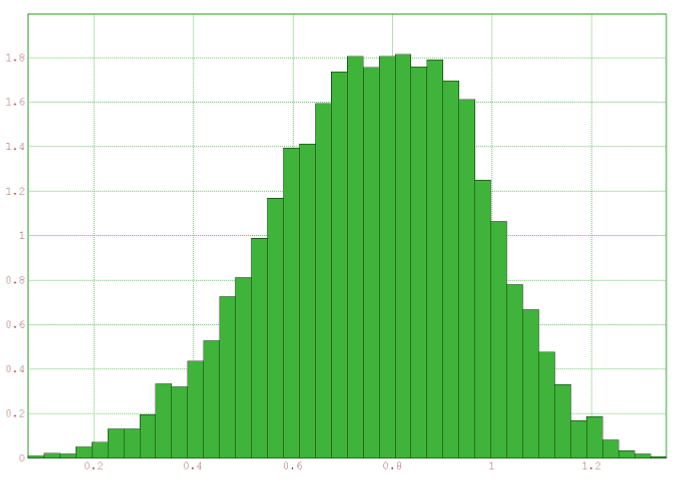
\includegraphics[scale=0.6]{content/Figure1.PNG} \\
\end{center}

\begin{Large}
\hspace{2mm} \colorbox{gray!20}{\textcolor{blue}{Représentation de lois continues, nombres de colonnes}}
\end{Large}

\hspace{3mm} Exemple: on tire 10 000 variables gaussiennes centrées réduites.\\
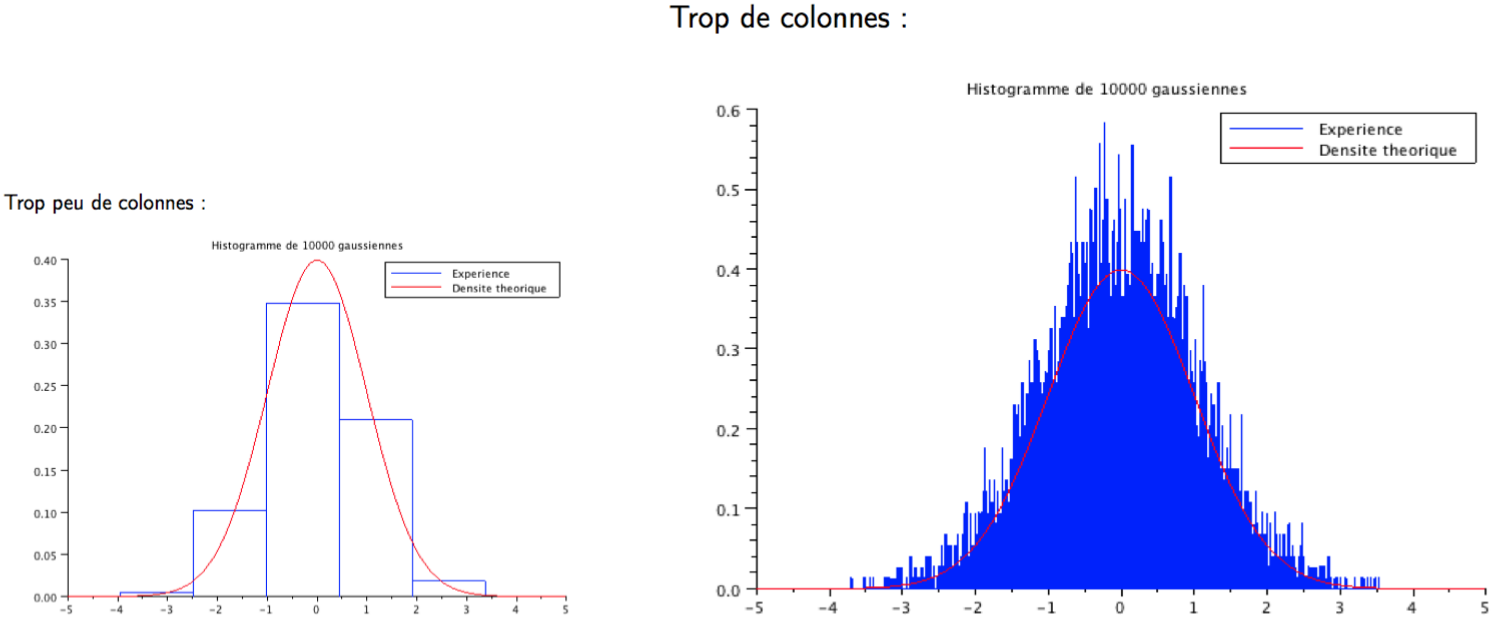
\includegraphics[scale=0.6]{content/Figure2.PNG} \\

\hspace{3mm} Idéal : prendre nombre de colonnes $\approx \sqrt{nombre \, de \, données}$ \\

\begin{center}
\begin{Large}
SIMULATION DES VARIABLES ALÉATOIRES \\
\end{Large}
\end{center}

{\textcolor{blue}{But:} Générer une $X$ variable aléatoire à partir d'une variable aléatoire uniforme $U \sim \mathcal{U} [0,1])$. \\

\vspace{1cm}

\begin{center}
\begin{Large}
SIMULATION DES VARIABLES ALÉATOIRES DISCRÈTES \\
\end{Large}
\end{center}

- Méthodes particulières \\
- Méthode générale. \\

\begin{Large}
\hspace{2mm} \colorbox{gray!20}{\textcolor{blue}{Loi de Bernoulli de paramètre $p \in [0,1]$}}
\end{Large}

\begin{center}
Si $U \in \mathcal{U} ([0,1])$ alors $X \mathds{1}_{\{U \leq p\}} \sim \mathcal{B} (p)$ \\
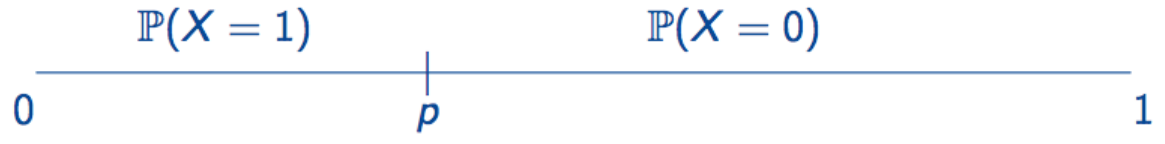
\includegraphics[scale=0.6]{content/Figure3.PNG}
\end{center}
En effet: $\mathbb{P} (X = 1) = \mathbb{P} (U \leq p) = \int_{0}^{1} \mathds{1}_{\{u \leq p\}} \mathrm{d}u = p$ \\

\begin{Large}
\hspace{2mm} \colorbox{gray!20}{\textcolor{blue}{Loi binomiale de paramètre $n \in \mathbb{N}^{*}$ et  $p \in [0,1]$}}
\end{Large}

\hspace{4mm} Si $U_{1}, ... U_{n}$ sont $n$ v.a. uniformes sur [0,1] dépendantes alors
\[ X = \mathds{1}_{\{U_{1} \leq p \}} + \dots + \mathds{1}_{\{U_{n} \leq p \}} = \sum \limits_{i=1}^{n} \mathds{1}_{\{U_{i} \leq p\}} \sim \beta (n,p) \]
En effet, les v.a. $\mathds{1}_{\{U_{i} \leq p\}}$, $1 \leq i \leq n$, sont Bernoulli de paramètre $p$ et indépendantes. \\

\begin{Large}
\hspace{2mm} \colorbox{gray!20}{\textcolor{blue}{Loi géométrique de paramètre $p \in ]0,1[$}}
\end{Large}

\hspace{4mm} C'est la loi du temps de 1er succès dans une suite d'expériences aléatoires indépendantes avec probabilité de succès $p$. Donc
\[ N = \inf \{ i \geq 1: U_{i} \leq p \} \sim \mathcal{G}éo(p) \]
Défaut : nombre moyen de v.a. uniformes utilisées égal à
$\mathbb{E} [N] = 1/p$ qui est grand pour des petites valeurs de $p$.\\

\begin{Large}
\hspace{2mm} \colorbox{gray!20}{\textcolor{blue}{Méthode avec une seule variable aléatoire uniforme}}
\end{Large}

\hspace{4mm} Si $U \sim \mathcal{U} ([0,1])$ alors $1+E \Big( \dfrac{\ln (U)}{\ln (1-p)} \Big)$ suit la loi géométrique de paramètre $p$. ($E(x)$ est la partie entière : $E(x) \leq x < E(x) + 1$.)\\

\begin{Large}
\hspace{2mm} \colorbox{gray!20}{\textcolor{blue}{Démonstration}}
\end{Large}
\hspace{4mm} Soit $X= 1+ E \Big(\dfrac{\ln (U)}{\ln (1-p)} \Big) $ et $k \in \mathbb{N}^{*}$: \\
\begin{align*}
\mathbb{P} (X = k) &= \mathbb{P} \Big( E \Big( \dfrac{\ln (U)}{\ln (1-p)} \Big) = k-1 \Big) \\
&= \mathbb{P} \Big( k-1 \leq \dfrac{\ln (U)}{\ln (1-p)} < k \Big) \\
&= \mathbb{P} (k \ln (1-p) < \ln (U) \leq (k-1) \ln (1-p)) \\
&= \mathbb{P} \big( (1-p)^{k} < U \leq (1-p)^{k-1} \big) \\
&= (1-p)^{k-1} - (1-p)^{k} \\
&= (1-p)^{k-1}p
\end{align*}

\vspace{1cm}

\begin{center}
\begin{Large}
SIMULATION DES VARIABLES ALÉATOIRES DISCRÈTES \\
\end{Large}
\end{center}

- Méthode par inversion de la fonction de répartition\\
- Méthodes particulières\\
- Méthode du rejet. \\

\begin{Large}
\hspace{2mm} \colorbox{gray!20}{\textcolor{blue}{Préliminaires}}
\end{Large}

\hspace{4mm} Soit $X$ unev.a. réelle de fonction de répartition $F$ définie par
\[ F(x) = \mathbb{P} (X \leq x)\]
$F$ est croissante, continue à droite et limitée à gauche en tout point de $\mathbb{R}$ et que $\underset{x\to - \infty}{\lim} F(x) =1$ \\%(cf. Cours 3, séance 1) \\
\vspace{1mm}
Si $X$ a une densité $f$ (c-à-d si $F(x) = \int_{- \infty}^{x} f(y) \mathrm{d}y$), \\
$F'(x) = f(x)$ en tout point où $f$ est continue. %(cf. Cours 3, séance 2)

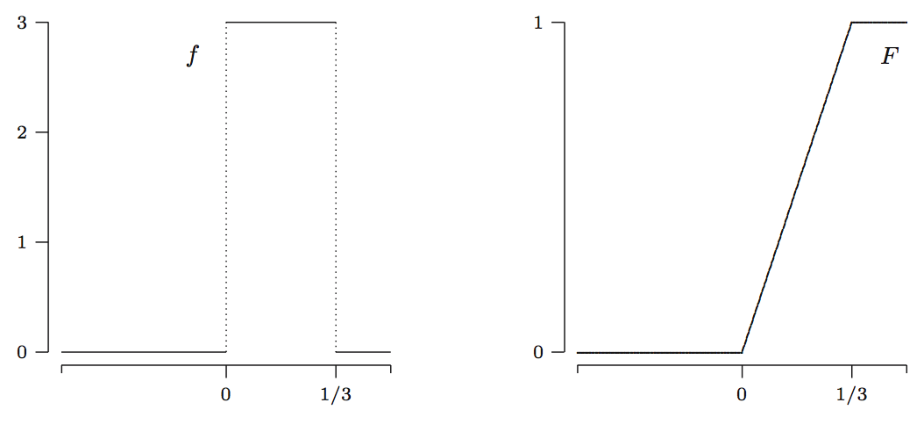
\includegraphics[scale=0.6]{content/Figure4.PNG}
\[ X \sim \mathcal{U} ([0,1/3]) \\
f(x) = 3 \mathds{1}_{[0,1/3]} (x), \,
F(x) = \left\{
\begin{array}{ll}
0 \hspace{8mm} si x <0 \\
3x \hspace{7mm} si 0 \leq x < 1/3 \\
1 \hspace{8mm} si x \geq 1/3

\end{array}
\right.  \]

%%%%%%%%%%%%%%%%%%%%%%%%%%%%%%%%%%%%%%%%%%%%%%%%%%%%%%%%%%%%%%%%%%%%%%%%%%%%%%%%
%%%%%%%%%%%%%%%%%%%%%%%%%%%%%%%%%%%%%%%%%%%%%%%%%%%%%%%%%%%%%%%%%%%%%%%%%%%%%%%%
%%%%%%%%%%%%%%%%%%%%%%%%%  partie de lecheguer  %%%%%%%%%%%%%%%%%%%%%%%%%%%%%%%%
%%%%%%%%%%%%%%%%%%%%%%%%%%%%%%%% FIN  %%%%%%%%%%%%%%%%%%%%%%%%%%%%%%%%%%%%%%%%%%
%%%%%%%%%%%%%%%%%%%%%%%%%%%%%%%%%%%%%%%%%%%%%%%%%%%%%%%%%%%%%%%%%%%%%%%%%%%%%%%%
\subsection{Méthode d’inversion de la fonction de répartition}

Si $U \sim \mathcal{U}([0,1])$ et si
$X$ a pour fonction de répartition $F$ alors $X$ et $F^{−1}(U)$ ont
même loi.\\

C’est évident si $F$ est continue et strictement croissante sur $\mathbb{R}$
car elle réalise alors une bijection de $\mathbb{R}$ sur $]0,1[$ et admet donc
un inverse $F^{−1}: ]0,1[\rightarrow \mathbb{R}$.\\

$Y:=F^{-1}(U)$ a alors la même loi que $X$:
$$\mathbb{P}(Y\leq x)=\mathbb{P}(F^{-1}(U)\leq x)=\mathbb{P}(U\leq F(x))=F(x).$$
En général, $F$ n’a pas d’inverse mais le résultat précédent reste
vrai si on prend l’inverse généralisé (quantile) de $F$ : $$F^{-1}(u):=\min\{x\in \mathbb{R}:F(x)\geq u\}$$

\begin{figure}[h]
\centering
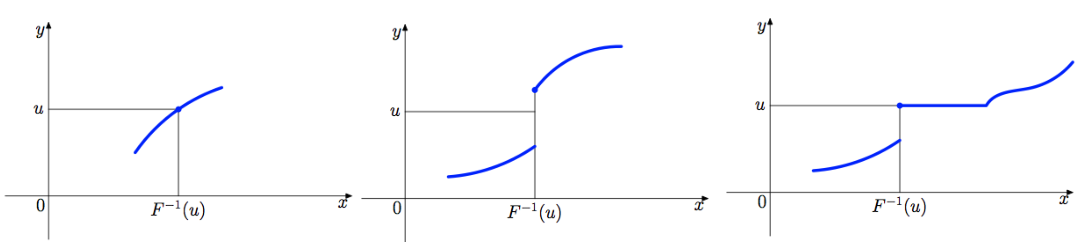
\includegraphics[width=13cm]{content/figfoncrep.PNG}

\end{figure}

\subsubsectionnn{Loi exponentielle}

$Y:=-\frac{\log U}{\lambda}$ suit la loi exponentielle de paramètre $\lambda>0$\\

En effet, $F(x)=1-\exp(-\lambda x)$ s'inverse en $F^{-1}(u)=-\frac{\log(1-u)}{\lambda}$ mais on observe que $1-U$ a même
loi que $U$.

\subsubsectionnn{Loi de Weibull}

Utilisée en fiabilité et caractérisée par sa «fonction de survie» $G(x)=1-F(x)=\exp(-x^{a}), a>0 \text{ paramètre },x\geq 0$.
\vspace{0.05cm}

On écrit que $X\sim Weib(a)$.
\vspace{0.5cm}

On observe que $U$ et $1 − U$ ont même loi et on trouve facilement que $Y:=(-\log U)^{1/a}$ suit la loi $Weib(a)$.

\subsubsectionnn{Loi de Cauchy $\mathcal{C}(a)$}
C’est la loi de densité $f(x)=\frac{1}{\pi}\frac{a}{x^2+a^2}, a>0 \text{ paramètre }, x\in\mathbb{R}$.\\
\vspace{0.05cm}

$F(x)=\frac{1}{\pi} \arctan(\frac{x}{a})+\frac{1}{2}$\\
\vspace{0.05cm}

Étant donné $u \in ]0,1[$, on cherche $x$ tel que $F(x) = u$ : $$F(x)=u\iff x=a\tan(\pi(u-1/2)).$$
Donc $Y:=a\tan(\pi(U-\frac{1}{2}))$ suit la loi de Cauchy de paramètre $a$.

\subsubsectionnn{Résumé (lois usuelles)}

$U\sim\mathcal{U}([0,1])$, $(U_i)$ suite de $v.a.i.i.d.$ suivant cette loi.

\begin{table}[h!]
\centering
\begin{tabular}{||c | c||}
\hline
Loi                             &   Méthode de simulation\\
\hline
Bernoulli $\mathcal{B}(p)$              &   $\mathds{1}_{\{U\leq p\}}$\\
\hline
Binomiale $\mathcal{B}(n,p)$            &   $\sum_{i=1}^{n}\mathds{1}_{\{U_i\leq p\}}$\\
\hline
Géométrique $\mathcal{Gé}\text{éo}(p)$  &   $1+E\big(\frac{\log(U)}{\log(1-p)}\big)$\\
\hline
Poisson $\mathcal{P}(\lambda)$          &   $\inf\{n\in\mathbb{N}:U_1\times U_2\times\dots\times U_{n+1}\leq e^{-\lambda}\}$\\
\hline
Uniforme $\mathcal{U}([a,b]))$          &   $a+(b-a)U$\\
\hline
Exponentielle $\mathcal{E}(\lambda)$    &   $-\frac{1}{\lambda}\log(U)$\\
\hline
Cauchy $\mathcal{C}(a)$                 &   $a\tan(\pi(U-\frac{1}{2}))$\\
\hline
Normale $\mathcal{N}(\mu,\sigma^2)$     &   $\mu+\sigma\sqrt{-2\log(U_1)}\cos(2\pi U_2)$\\
\hline
\end{tabular}

\end{table}

\subsubsectionnn{Autres exemples:}
\textbullet Si $X$ suit la loi de Laplace centrée réduite (loi «double
exponentielle») :$$f(x)=\frac{1}{2}e^{-|x|},\quad\mathrm{     }\quad F(x)=\frac{1}{2}\big(1+\sign(x)(1-e^{-|x|})\big)$$
elle a la même loi que $$Y=-\sign(U)\log(1-2|U|)\quad\mathrm{   \text{où}  }\quad U\sim\mathcal{U}([-0.5,0.5]).$$

\textbullet Si $X$ suit la loi de Gumbel (centrée réduite) :
$$f(x=e^{-(x+e^{-x})}), \quad\mathrm{     }\quad F(x)=e^{-e^{-x}}$$ elle a la même loi que
$$Y=-\log(-\log(U))\quad\mathrm{   \text{où}  }\quad U\sim\mathcal{U}([0,1]).$$
Cette loi sert pour décrire le maximum d’une série de données
(par ex. niveau d’une rivière).

\subsection{Illustration de la méthode d'inversion de la fonction de répartition}



\begin{figure}[h]
\centering
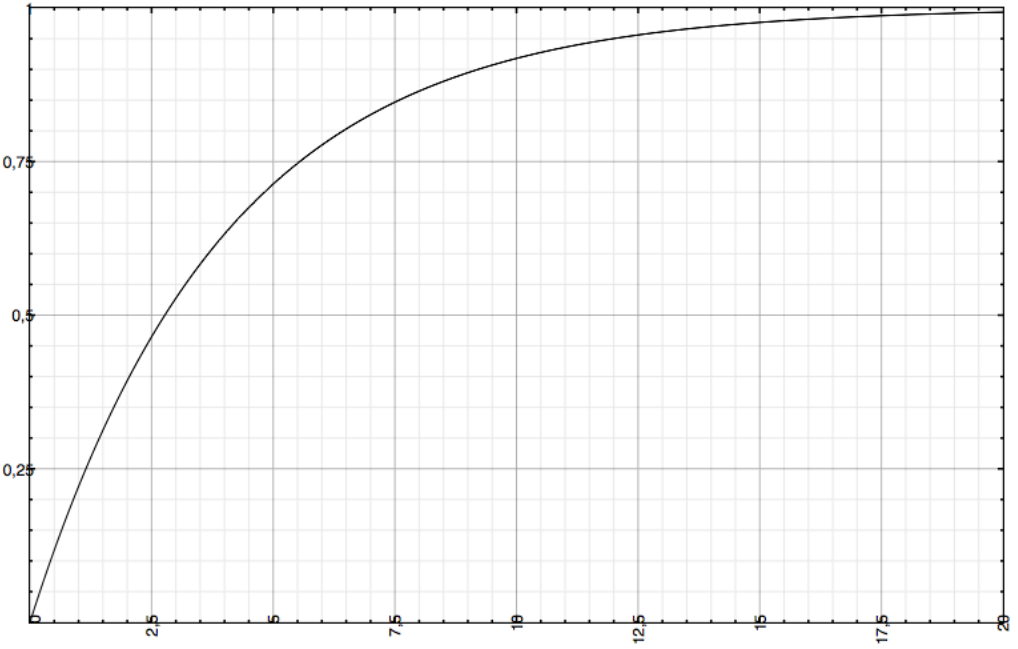
\includegraphics[width=7.5cm]{content/foncrepexp.PNG}
\caption{Loi exponentielle:\\$F(x)=(1-e^{-0.25x})\mathds{1}_{\mathbb{R}_{+}}(x)$\\$f(x)=0.25e^{-0.25x}$ }
\end{figure}


\begin{figure}[h]
\centering
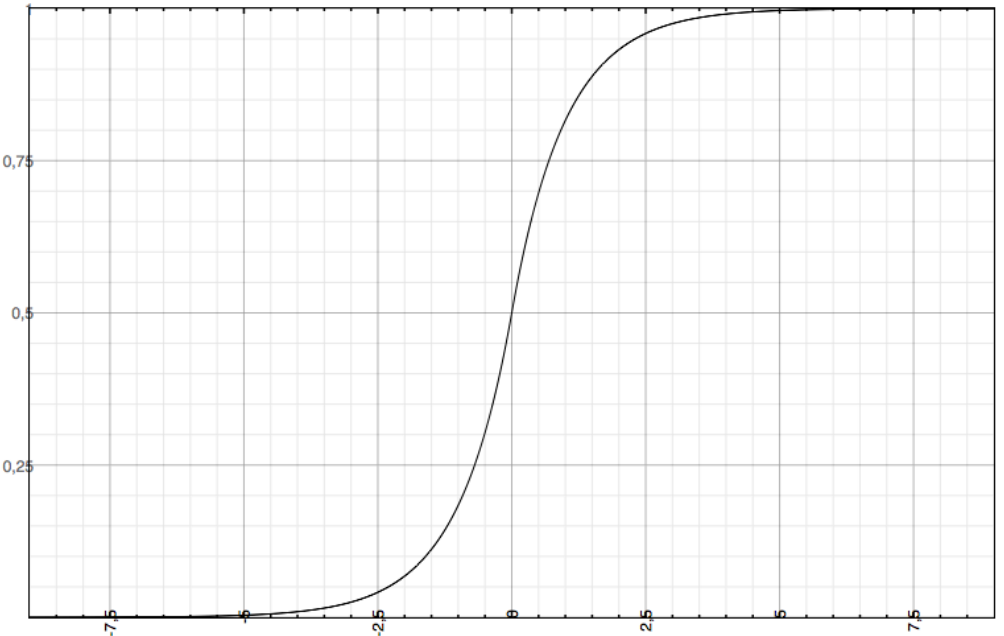
\includegraphics[width=7.5cm]{content/lap.PNG}
\caption{Loi de Laplace:\\$F(x)=0.5\big(1+\sign(x)(1-e^{-|x|})\big)$\\$f(x)=0.5e^{-|x|}$ }
\end{figure}

\begin{figure}[h]
\centering
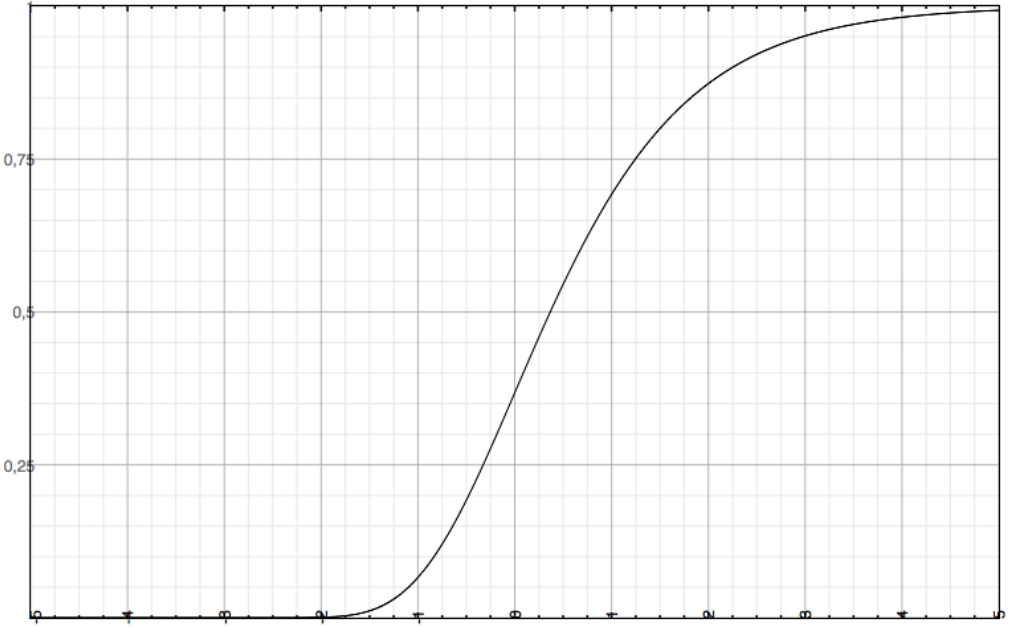
\includegraphics[width=7.5cm]{content/gumbel.PNG}
\caption{Loi de Gumbel:\\$F(x)=e^{-e^{-x}}$\\$f(x)=e^{-(x+e^{-x})}$ }
\end{figure}



















\iffalse
\section{Loi d’une variable aléatoire à densité}\label{chap:2}
Nous avons introduit le concept de fonctions de densité de probabilité et de masse de probabilité de variables aléatoires
dans le chapitre précédent. Dans ce chapitre, nous introduisons des distributions de probabilité standard discrètes et
continues communes qui sont largement utilisées pour des applications pratiques ou pour construire des méthodes
statistiques. Supposons que nous soyons intéressés à déterminer la probabilité d'un certain événement. La détermination
des probabilités dépend de la nature de l’étude et des diverses conditions qui l’affectent. Par exemple, la détermination
de la probabilité d'une tête lors du lancement d'une pièce est différente de la détermination de la probabilité de pluie
l'après-midi. On peut supposer que certaines fonctions mathématiques peuvent être définies qui décrivent le comportement
des probabilités dans différentes situations. Ces fonctions ont des propriétés spéciales et décrivent comment les
probabilités sont réparties dans différentes conditions. Nous avons déjà appris qu'elles sont appelées fonctions de
distribution de probabilité. La forme de ces fonctions peut être simple ou compliquée selon la nature et la complexité du
phénomène considéré. Rappelons d'abord et élargissons la définition des variables aléatoires indépendantes et
identiquement distribuées:

\theoremstyle{definition}
\begin{definition}
    Les variables aléatoires $X_1, X_2,\dots, X_n$ sont appelées indépendantes et identiquement distribuées (iid) si
    les  $X_i (i = 1,2,\dots, n)$ ont la même fonction de répartition marginale $F (x)$ et si elles sont mutuellement
    indépendantes.
\end{definition}

\begin{example}
    Supposons qu'un chercheur planifie une enquête sur le poids des nouveau-nés dans un pays. Le chercheur contacte au
    hasard $10$ hôpitaux avec une maternité et leur demande de sélectionner au hasard $20$ des nouveau-nés (pas de
    jumeaux) nés au cours des $6$ derniers mois et enregistre leur poids. L'échantillon est donc composé
    de $10 \times 20 = 200$ poids de bébé. Les hôpitaux et les bébés étant choisis au hasard, le poids des bébés n'est
    donc pas connu à l'avance. Les $200$ poids peuvent être désignés par les variables aléatoires $X_1, X_2,\dots, X_{200}$.
    Notez que les poids $X_i$ sont des variables aléatoires car, en fonction de la taille de la population, différents
    échantillons constitués de $200$ bébés peuvent être sélectionnés au hasard. En outre, les poids des bébés peuvent
    être considérés comme \textit{stochastiquement indépendants} (un exemple de poids dépendant stochastiquement serait
    le poids des jumeaux s’ils sont inclus dans l’échantillon). Après avoir collecté les poids de $200$ bébés, le
    chercheur dispose d'un échantillon de $200$ valeurs réalisées (c'est-à-dire les poids en grammes). Les valeurs
    sont maintenant connues et désignées par $x_1, x_2,\dots, x_{200}$.
\end{example}

\subsection{Distributions discrètes standard}

Tout d'abord, nous discutons de certaines distributions standard pour les variables aléatoires discrètes.

\subsubsection{Loi uniforme discrète}

La distribution uniforme discrète suppose que tous les résultats possibles ont une probabilité d'occurrence
égale. Une définition plus formelle est donnée comme suit:

\theoremstyle{definition}
\begin{definition}
    On dit qu'une variable aléatoire discrète $ X $ avec $ k $ résultats possibles $ x_1, x_2, ..., x_k $ suit une
    distribution \textbf{uniforme} discrète si la fonction de masse de probabilité de $X$ est donnée par
    \begin{equation}
        P(X=x_i)=\frac{1}{k}, \forall i=1, 2,\dots,k.
    \end{equation}
\end{definition}
Si les résultats sont les nombres naturels $ x_i = i (i = 1,2, ..., k) $, la moyenne et la variance de $ X $ sont
obtenues comme
\begin{align}
    E(X) &= \frac{k+1}{2}\\
    Var(X) &=\frac{1}{12}(k^2-1)
\end{align}

\begin{example}
    Si nous lançons un dé non pipé, les résultats "1", "2",\dots, "6" ont une probabilité égale de se produire, et donc,
    la variable aléatoire $X$ "nombre de points observés sur la surface supérieure du dé" a une distribution discrète
    uniforme avec une fonction de masse
    $$P(X=i)=\frac{1}{6}, \text{ pour tout } i=1,2,\dots,6.$$
    La moyenne et la variance de $X$ sont
    \begin{align*}
        E(X) &=\frac{6+1}{2}=3.5,\\
        Var(X) &=\frac{1}{12}(6^2-1)=35/12.
    \end{align*}
    \begin{SCfigure}[0.8][h]
        \caption{Distribution de fréquence de $1000 $ nombres aléatoires uniformes
discrets générés avec comme résultats possibles $ (2,5,8,10) $}
        \label{fig:frecunif}
        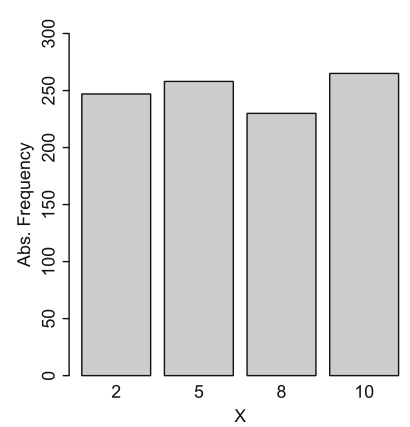
\includegraphics[width=0.4\textwidth]{content/frecunif.PNG}
    \end{SCfigure}
\end{example}
En utilisant la fonction sample () dans R, il est facile de générer des nombres aléatoires à partir d'une distribution
uniforme discrète. La commande suivante génère un échantillon aléatoire de taille 1000 à partir d'une distribution
uniforme avec les quatre résultats possibles 2, 5, 8, 10 et trace un graphique à barres des nombres observés.
L'utilisation de la fonction set.seed () permet de reproduire à tout moment les nombres aléatoires générés. Il est
nécessaire d'utiliser l'option replace = TRUE pour simuler des tirages avec remplacement, c'est-à-dire pour garantir
qu'une valeur puisse se produire plus d'une fois.

\begin{verbatim}
    set.seed(123789)
    x <- sample(x=c(2,5,8,10), size=1000, replace=T,
    prob=c(1/4,1/4,1/4,1/4))
    barchart(table(x), ylim=c(0,300))
\end{verbatim}

Un diagramme à barres de la distribution de fréquence des 1000 nombres échantillonnés avec les résultats possibles
(2, 5, 8, 10) en utilisant la distribution uniforme discrète est donné à la Fig. \ref{fig:frecunif}. Nous voyons que les 1000 nombres
aléatoires générés ne sont pas exactement uniformément distribués, par ex. les nombres 5 et 10 se produisent plus
souvent que les nombres 2 et 8. En fait, ils ne sont qu'approximativement uniformes. Nous nous attendons à ce que
l'écart par rapport à une distribution uniforme parfaite diminue à mesure que nous générons de plus en plus de nombres
aléatoires, mais ne sera probablement jamais nul pour un nombre fini de tirages. Les nombres aléatoires reflètent la
situation pratique selon laquelle une distribution d'échantillon n'est qu'une approximation de la distribution
théorique à partir de laquelle l'échantillon a été tiré.

\subsubsection{Distribution dégénérée}

\theoremstyle{definition}
\begin{definition}
    Une variable aléatoire $ X $ a une distribution dégénérée à $ a $, si $ a $ est le seul résultat possible
    avec $ P (X = a) = 1 $. La fonction de répartition dans un tel cas est donnée par
    $$F(x) = \begin{cases} 0 & \mbox{si   } x<a\\ 1 & \mbox{si } x\geq a.\end{cases}$$
\end{definition}
De plus, $E (X) = a$ et $Var (X) = 0$.\\
La distribution dégénérée indique qu'il n'y a qu'un seul résultat fixe possible, et donc, aucun hasard n'est impliqué.
Il s'ensuit que nous avons besoin d'au moins deux résultats possibles différents pour avoir un caractère aléatoire
dans les observations d'une variable aléatoire ou d'une expérience aléatoire. La distribution de Bernoulli est une
telle distribution où il n'y a que deux résultats, par ex. succès et échec ou masculin et féminin. Ces résultats sont
généralement désignés par les valeurs «0» et «1».

\subsubsection{La distribution de Bernoulli}

\theoremstyle{definition}
\begin{definition}
    Une variable aléatoire $ X $ a une distribution de Bernoulli si la fonction de masse de X est donnée comme
    $$P(X=x) = \begin{cases} p & \mbox{si   } x=1\\ 1-p & \mbox{si } x=0.\end{cases}$$
\end{definition}
La fonction de répartition de $X$est:

$$F(x) = \begin{cases} 0 & \mbox{si   } x<0\\ 1-p & \mbox{si } 0\leq x<1\\1 & \mbox{si   } x\geq 1.\end{cases}$$

La moyenne (espérance) et la variance d'une variable aléatoire de Bernoulli sont calculées comme suit:
\begin{equation}\label{eq:esp}
    E(X)=1.p+0.(1-p)=p
\end{equation}

\begin{equation}\label{eq:var}
    Var(X)=(1-p)^2.p+(0-p)^2.(1-p)=p(1-p),
\end{equation}
respectivement.\\

Une distribution de Bernoulli est utile lorsqu'il n'y a que deux résultats possibles, et notre intérêt réside dans
l'un des deux résultats, par ex. si un client achète un certain produit ou non, ou si un ouragan frappe une île ou
non. Le résultat d'un événement $ A $ est généralement codé comme $ 1 $, ce qui se produit avec la probabilité $ p $.
Si l'événement d'intérêt ne se produit pas, c'est-à-dire que l'événement complémentaire $\bar{A}$ se produit, le
résultat est codé comme $ 0 $, ce qui se produit avec la probabilité $ 1 - p $. Donc $ p $ est la probabilité que
l'événement d'intérêt $ A $ se produise.

\begin{example}
    Une entreprise organise un tirage au sort à la fin de l'année. Il y a au total $300$ billets de loterie, et
    $50$ d'entre eux sont marqués comme des billets gagnants. L'événement $ A $ d'intérêt est le «ticket gagne»
    (codé $ X = 1 $), et la probabilité $ p $ d'avoir un ticket gagnant est a priori (c'est-à-dire avant qu'un ticket
    de loterie soit tiré)
    \begin{equation*}
        P(X=1)=\frac{50}{300}=\frac{1}{6}=p
        \quad\mathrm{  et }\quad
        P(X=0)=\frac{250}{300}=\frac{5}{6}=1-p.
    \end{equation*}
    Selon (\ref{eq:esp}) et (\ref{eq:var}), la moyenne (espérance) et la variance de $ X $ sont
    \begin{equation*}
        E(X)=\frac{1}{6}
        \quad\mathrm{  et }\quad
        Var(X)=\frac{1}{6} . \frac{5}{6}=\frac{5}{36} \text{  respectivement.}
    \end{equation*}
\end{example}

\subsubsection{Distribution binomiale}

Considérons $ n $ essais indépendants ou répétitions d'une expérience de Bernoulli. Dans chaque essai ou répétition,
nous pouvons observer $ A $ ou $ \bar{A} $. A la fin de l'expérience, nous avons ainsi observé $ A $ entre $ 0 $ et
$ n $ fois. Supposons que nous nous intéressions à la probabilité que $ A $ se produise $ k $ fois, alors la
distribution binomiale est utile.

\begin{example}
    Considérons une expérience de lancer de pièces où une pièce est lancée dix fois et l'événement d'intérêt est
    $ A =$ «face» . La variable aléatoire $ X $ "nombre de face dans $ 10 $ expériences" a les résultats possibles
    $ k = 0,1, ..., 10 $. Une question d'intérêt peut être: Quelle est la probabilité qu'un visage se produise dans
    $7$ des $10$ essais; ou dans $5$ essais sur $10$? Nous supposons que l'ordre dans lequel les faces (et les piles)
    apparaissent n'est pas intéressant, seul le nombre total de face est intéressant.
\end{example}

La distribution binomiale répond à ces questions. Cette distribution peut être motivée soit par une répétition
d'expériences de Bernoulli $ n $ (comme dans l'exemple de lancer de pièces ci-dessus), soit par le modèle de
l'urne: supposons qu'il y ait des boules blanches $ M $ et $ N - M $ noires dans l'urne. Supposons que n balles soient
tirées au hasard de l'urne, la couleur de la balle est enregistrée et la balle est replacée dans l'urne
(échantillonnage avec remise). Soit $ A $ l'événement auquel une boule blanche est tirée de l'urne. La probabilité
de $ A $ est $ p = M / N $ (la probabilité de tirer une boule noire est $ 1 - p = (N - M) / N) $. Puisque les balles
sont tirées avec remplacement, ces probabilités ne changent pas d'un tirage à l'autre. De plus, soit $ X $  la variable
aléatoire comptant le nombre de boules blanches tirées de l'urne dans les expériences $ n $. Puisque l'ordre des
couleurs résultantes des boules n'est pas intéressant dans ce cas, il existe des combinaisons $\binom{n}{k} $ où $ k $
boules sont blanches et $ n - k $ boules  sont noires. Puisque les boules sont tirées avec remplacement, chaque
résultat des  $ n $ expériences est indépendant de tous les autres. La probabilité que $ X = k, k = 0,1, ..., n $,
puisse donc être calculée comme

\begin{equation}\label{eq:binomial}
P(X=k)=\binom{n}{k}p^k(1-p)^{n-k} \quad\mathrm{   }\quad (k=0,1,\dots,n).
\end{equation}

Veuillez noter que nous pouvons utiliser le produit $ p^k(1-p)^{n-k} $ car les tirages sont indépendants.
Le coefficient binomial $ \binom{n}{k} $ est nécessaire pour compter le nombre d'ordres possibles des boules noires
et blanches.

\theoremstyle{definition}
\begin{definition}
    On dit qu'une variable aléatoire discrète $X$ suit une distribution binomiale de paramètres $ n $ et $ p $ si
    sa fonction de masse est donnée par (\ref{eq:binomial}). Nous écrivons également $ X \sim B (n; p) $. \\
    La moyenne et la variance d'une variable aléatoire binomiale $X$ sont données par
    \begin{align}
        E(X) &= np,\\
        V(X) &= np(1-p).
    \end{align}
\end{definition}

\begin{remark}
    Une variable aléatoire de Bernoulli est donc $B(1; p)$ distribuée.
\end{remark}

\begin{example}\label{ex:2.5}
    Supposons que nous lançons un dé pipé $50$ fois avec la probabilité de pile $p_ {pile} = 0,6$.
    Nous avons donc affaire à une distribution $B(50,0.6)$ qui peut être tracée à l'aide de la commande \emph{dbinom}.
    Le préfixe \mathcal{d} signifie «densité».


\begin{SCfigure}[0.8][h]
    \caption{fonction de masse d'une distribution $B(50, 0.6)$}
    \label{fig:binomplot}
    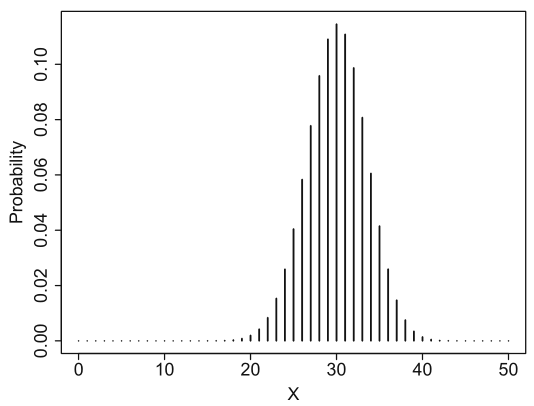
\includegraphics[width=0.4\textwidth]{content/binomplot.PNG}
\end{SCfigure}

\begin{verbatim}
    n <- 50
    p <- 0.6
    k <- 0:n
    pmf <- dbinom(k,n,p)
    plot(k,pmf, type=h)
\end{verbatim}

    Un tracé de la fonction de masse d'une distribution binomiale avec $ n = 50 $ et $ p = 0,6 $
    (c'est-à-dire $ B (50,0,6) $) est donné sur la Figure \ref{fig:binomplot}.\\
    Notons que nous pouvons également calculer la fonction de répartition avec $ R $. Nous pouvons utiliser la
    commande \textit {pbinom (x, n, p)}, où le préfixe $ p $ signifie probabilité, pour calculer la fonction de
    répartition à tout point. Par exemple, supposons que nous nous intéressions à $ P (X \geq 30) = 1 - F (29) $,
    c'est-à-dire la probabilité d'observer trente piles ou plus; puis on écrit

    \begin{verbatim}
        1-pbinom(29,50,0.6)
        [1] 0.5610349
    \end{verbatim}

De même, nous pouvons déterminer des quantiles. Par exemple, le $ 80\% $ quantile $ q $ qui décrit
    que $ P (X \leq q) ≥ 0,8 $ peut être obtenu par la commande \textit {qbinom(q, n, p)} comme suit:
\begin{verbatim}
    qbinom(0.8,50,0.6)
    [1] 33
\end{verbatim}
    Si nous voulons générer $ 100 $ réalisations aléatoires  à partir d'une distribution $ B (50,0.6) $,
    nous pouvons utiliser la commande \textit{rbinom}.
    \begin{verbatim}
        rbinom(100,50,0.6)
    \end{verbatim}
\end{example}
La distribution binomiale a de belles propriétés. L'une d'elles est décrit dans le théorème suivant:
\theoremstyle{theorem}
\begin{theorem}
    Soit $ X \sim B (n; p) $ et $ Y \sim B (m; p) $ et supposons que $ X $ et $ Y $ sont (stochastiquement)
    indépendants. Alors
    \begin{equation}
        X+Y\sim B(n+m;p).
    \end{equation}
\end{theorem}
Ceci est intuitivement clair puisque nous pouvons interpréter ce théorème comme décrivant la combinaison additive
de deux expériences binomiales indépendantes avec $ n$ et $m$ essais, avec une probabilité égale $ p $, respectivement.
Puisque chaque expérience binomiale est une série d'expériences Bernoulli indépendantes, cela équivaut à une série
d'essais Bernoulli indépendants $ n + m $ avec une probabilité de succès constante $ p $ qui à son tour équivaut à
une distribution binomiale avec  $ n + m $ essais

\subsubsection{Distribution de Poisson}
Considérons une situation dans laquelle le nombre d'événements est très élevé et la probabilité de succès est
très faible: par exemple, le nombre de particules alpha émises par une substance radioactive entrant dans une
région particulière dans un court intervalle de temps donné. Notez que le nombre de particules alpha émises est
très élevé mais seules quelques particules sont transmises à travers la région dans un court intervalle de temps
donné. Quelques autres exemples où les distributions de Poisson sont utiles sont le nombre de cas de grippe dans un
pays en un an, le nombre de tempêtes tropicales dans une zone donnée en un an, ou le nombre de bactéries trouvées dans
une enquête biologique

\theoremstyle{definition}
\begin{definition}
    On dit qu'une variable aléatoire discrète $ X $ suit une distribution de Poisson de paramètre
    $ \lambda> 0 $ si sa fonction de masse est donnée par
    \begin{equation}\label{eq:26}
        P(X=x)=\frac{\lambda^x}{x!}\exp(-\lambda) \quad\mathrm{    }\quad   (x=0,1,2,\dots).
    \end{equation}
\end{definition}
Nous écrivons également $ X \sim Po(\lambda) $. La moyenne et la variance d'une variable aléatoire de Poisson
sont identiques:
$$E(X)=Var(X)=\lambda.$$

\begin{example}
    Supposons qu'un pays subisse en moyenne X $ = 4 $ tempêtes tropicales par an. Ensuite, la probabilité de
    souffrir de seulement deux tempêtes tropicales est obtenue en utilisant la distribution de Poisson comme

    $$P(X=2)=\frac{\lambda^x}{x!}\exp(-\lambda)=\frac{4^2}{2!}\exp(-4)=0.146525$$

    Si nous sommes intéressés par la probabilité que pas plus de $2$ tempêtes soient subies, alors nous pouvons
    appliquer les règles (\ref{sub-eq-1:8})-(\ref{sub-eq-1:14}) du Chap. \ref{chap:1}:
    $P (X \leq 2) = P (X = 2) + P (X = 1) + P (X = 0) = F (2) = 0,2381033$.
    Nous pouvons calculer $P (X = 1)$ et $P (X = 0)$ à partir de (\ref{eq:26}) ou en utilisant $R$. Semblable à
    l'exemple \ref{ex:2.5}, nous utilisons le préfixe $d$ pour obtenir la fonction de masse  et le préfixe $p$
    pour travailler avec la fonction de répartition, c'est-à-dire que nous pouvons utiliser \emph{dpois(x, \lambda)}
    et $  ppois(x, \lambda)$
    pour déterminer $P (X = x)$ et $P(X \leq x)$, respectivement.

    \begin{verbatim}
        dpois(2,4) + dpois(1,4) + dpois(0,4)
        [1] 0.2381033
        ppois(2,4)
        [1] 0.2381033
    \end{verbatim}
\end{example}

\subsubsection{Distribution géométrique}

Considérons une situation dans laquelle nous souhaitons déterminer combien d'essais Bernoulli indépendants sont
nécessaires jusqu'à ce que l'événement d'intérêt se produise pour la première fois. Par exemple, nous pouvons être
intéressés par le nombre de billets à acheter dans une tombola jusqu'à ce que nous gagnions pour la première fois, ou
le nombre de médicaments différents pour tenter de lutter avec succès contre une migraine sévère, etc. La distribution
géométrique peut être utilisée pour déterminer la probabilité que l'événement d'intérêt se produit au $k$ième procès
pour la première fois.

\theoremstyle{definition}
\begin{definition}
    On dit qu'une variable aléatoire discrète $X$ suit une distribution géométrique de paramètre $p$ si sa
    fonction de masse est donnée par
    \begin{equation}\label{eq:27}
        P(x=k)=p(1-p)^{k-1} \quad\mathrm{  ,  }\quad k=1,2,3,\dots
    \end{equation}
\end{definition}
La moyenne (espérance) et la variance sont respectivement données par $E (X) = 1/p$ et $Var (X) = 1/p (1/p  -  1)$.
\begin{example}
Prenons une expérience où une pièce est lancée jusqu'à ce que  «face» soit obtenue pour la première fois.
La probabilité d'obtenir face est de $p = 0,5$ pour chaque lancer. En utilisant (\ref{eq:27}),
nous pouvons déterminer les probabilités suivantes:
    \begin{align*}
        P(X=1) &=0.5\\
        P(X=2) &=0.5(1-0.5)=0.25\\
        P(X=3) &=0.5(1-0.5)^2=0.125\\
        P(X=4) &=0.5(1-0.5)^3=0.0625\\
        \text{       }\dots \text{    }  \dots
    \end{align*}
\end{example}
En utilisant $R$, nous pouvons déterminer la dernière probabilité de $P(X = 4)$ comme suit:
\begin{verbatim}
    dgeom(3,0.5)
\end{verbatim}
Notez que la définition de $X$ dans $R$ diffère légèrement de notre définition. Dans $R$, $k$ est le nombre d'échecs
avant le premier succès. Cela signifie que nous devons spécifier $k - 1$ dans la fonction \emph{dgeom} plutôt que $k$.
La moyenne et la variance de ce paramétrage sont
$$E(X)=\frac{1}{0.5}=2\quad\mathrm{;    }\quad Var(X)=\frac{1}{0.5}\bigg(\frac{1}{0.5}-1\bigg) =2.     $$

\subsection{Distributions continues standard}

Maintenant, nous discutons de certaines distributions de probabilité standard de variables aléatoires (absolument)
continues. Les caractéristiques des variables aléatoires continues sont que le nombre de résultats possibles est
infiniment infini et qu’elles ont une fonction de distribution continue $F(x)$. Il s'ensuit que les probabilités
ponctuelles sont nulles, c'est-à-dire $P(X = x) = 0$. De plus, nous supposons qu'il existe une fonction de densité
unique $f$, telle que $F(x)= \int_{-\infty}^{x}f(t)dt$.

\subsubsection{Distribution uniforme continue}

Un analogue continu de la distribution uniforme discrète est la distribution uniforme continue sur un intervalle
fermé dans $\mathbb{R} $.

\theoremstyle{definition}
\begin{definition}
    On dit qu'une variable aléatoire continue X suit une distribution uniforme (continue) dans l'intervalle $[a, b]$,
    c'est-à-dire $X \sim U(a,b)$,  si sa fonction de densité de probabilité est donnée par

    $$f(x) = \begin{cases} \frac{1}{b-a} & \mbox{si   } a\leq x\leq b\quad\mathrm{   }\quad (a<b)\\
                            0 & \mbox{sinon. }\end{cases}$$

\end{definition}
La moyenne est la variance de $X\sim U(a,b)$ sont
$$E(X)=\frac{a+b}{2} \quad\mathrm{ et }\quad Var(X)=\frac{(b-a)^2}{12},$$ respectivement.

\begin{example}
    Supposons qu'un train arrive régulièrement dans une station de métro toutes les 10 minutes. Si un passager arrive
    à la gare sans connaître l'horaire, le temps d'attente pour prendre le train est uniformément réparti avec la
    densité
    $$f(x) = \begin{cases} \frac{1}{10} & \mbox{si   } 0\leq x\leq 10\\
    0 & \mbox{sinon. }\end{cases}$$
    Le temps d'attente «moyen» est $E(X) = (10 + 0)/2 = 5 min$. La probabilité d'attendre le train pendant moins
    de $3min$ est évidemment de $0,3$ (ou $30\%$) qui peut être calculée dans R à l'aide de la
    commande $punif(x, a, b)$
    \begin{verbatim}
        punif(3,0,10)
    \end{verbatim}
\end{example}

\subsubsection{Distribution normale}
La distribution normale est l'une des distributions les plus importantes utilisées en statistique. Le nom a été donné
par Carl Friedrich Gauss (1777–1855), un mathématicien, astronome, géodésiste et physicien allemand qui a observé que
les mesures en géodésie et en astronomie s'écartent de manière aléatoire et symétrique de leurs vraies valeurs.
La distribution normale est donc aussi souvent appelée distribution gaussienne.

\theoremstyle{definition}
\begin{definition}
    On dit qu'une variable aléatoire $X$ suit une distribution normale de paramètres $\mu$ et $\sigma^2$ si sa
    densité de probabilité est donnée par
    \begin{equation}\label{eq:gauss}
        f(x)=\frac{1}{\sigma\sqrt{2\pi}}\bigg(-\frac{(x-\mu)^2}{2\sigma^2}\bigg); \quad\mathrm{   }\quad
        -\infty<x<\infty,-\infty<\mu<\infty,\sigma^2>0.
    \end{equation}
\end{definition}
On écrit $X\sim N(\mu,\sigma^2)$. La moyenne et la variance de $X$ sont
$$E(X)=\mu;\quad\mathrm{  et }\quad Var(X) =\sigma^2$$ respectivement. si $\mu=0$ et $\sigma^2=1$, alors $X$ suit une
\textbf{loi normale centrée réduite}(loi normale standard), $X\sim N(0,1)$. La densité de probabilité d'une
distribution normale standard est donnée par $$\phi(x)=\frac{1}{\sqrt{2\pi}}\exp(-\frac{x^2}{2});\quad\mathrm{   }\quad
-\infty<x<\infty.$$

La densité d'une distribution normale a son maximum (voir Fig. \ref{fig:pdfgauss} ) à $x = \mu$. La densité est également symétrique
autour de $\mu$. Les points d'inflexion de la densité sont à $(\mu - \sigma)$ et $(\mu + \sigma)$ (Fig. \ref{fig:pdfgauss}).
Un $\sigma$ inférieur indique une concentration plus élevée autour de la moyenne $\mu$. Un $\sigma$ plus élevé
indique une densité plus plate (Fig. \ref{fig:pdfsgauss} ).\\
La fonction de répartition de $X\sim N(\mu,\sigma^2)$ est
\begin{equation}\label{eq:frgauss}
    F(x)=\int_{-\infty}^{x}\phi(t)dt
\end{equation}
qui est souvent désignée par $\Phi(x)$. La valeur de $\Phi(x)$ pour différentes valeurs de x peut être obtenue avec $R$.
Par exemple,

\begin{figure}[h]
    \centering
    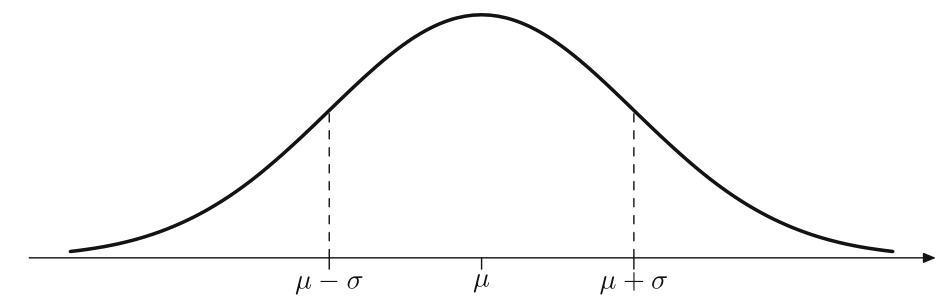
\includegraphics[width=0.5\textwidth]{content/pdfgauss}
    \caption{Densité de probabilité d'une distribution normale}
    \label{fig:pdfgauss}
\end{figure}

\begin{figure}[h]
    \centering
    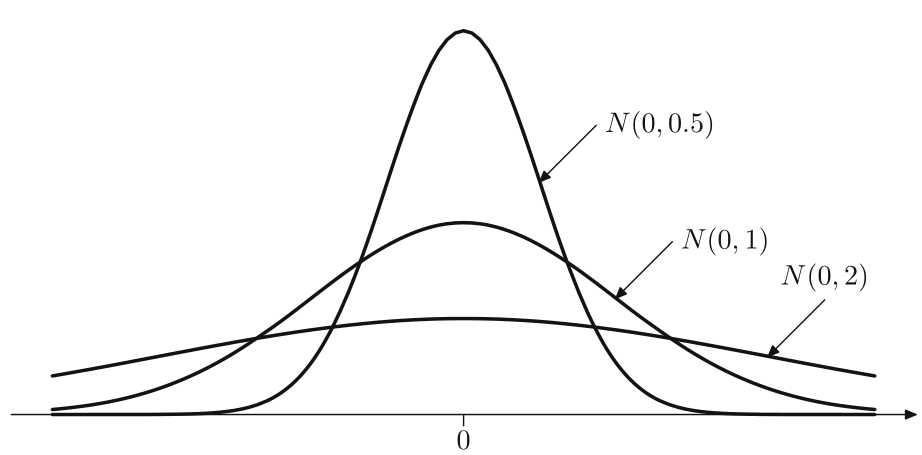
\includegraphics[width=0.5\textwidth]{content/pdfsgauss}
    \caption{Densité de probabilité des distributions $N(0;2)$, $N(0;1)$ et $N(0;0.5)$}
    \label{fig:pdfsgauss}
\end{figure}

\begin{verbatim}
    pnorm(1.96, mean = 0, sd = 1)
\end{verbatim}
calcule $\Phi(1,96)$ comme environ $0,975$. Cela signifie, pour une distribution normale standard, la
probabilité $P(X ≤ 1,96) \approx 0,975$.

\begin{remark}
    Il n'y a pas de formule explicite pour résoudre l'intégrale dans l'équation. (\ref{eq:frgauss}).
    elle doit être résolue par des méthodes numériques (ou informatiques). C'est la raison pour laquelle les
    tableaux de fonction de répartition sont présentés dans presque tous les manuels de Statistiques.
\end{remark}


Lorem ipsum dolor sit amet, consectetur adipiscing elit. Mauris vel nunc ultricies, lobortis leo a, mattis sapien. Duis nec sapien a diam sollicitudin consectetur. Etiam magna lorem, vulputate at fermentum sed, hendrerit nec metus. Integer ut nunc elit. Cras tristique finibus porttitor. Aliquam fringilla ipsum eget condimentum vehicula. Sed ac tellus ac erat sagittis ullamcorper quis a leo. Nulla sed elit tincidunt, posuere velit sed, fringilla quam. Praesent facilisis eros nec leo luctus, in mattis quam rhoncus.

Phasellus lorem erat, aliquet at dapibus in, egestas at justo. Cras a lectus eget libero faucibus cursus. Nulla et facilisis dui. In orci odio, faucibus a ultricies eu, finibus ut massa. Praesent ac sem volutpat, tempor risus quis, aliquet turpis. In hac habitasse platea dictumst. Vestibulum laoreet, justo id semper eleifend, augue dui molestie ligula, id varius erat mi a quam. Etiam cursus, justo ac lobortis viverra, nibh neque faucibus nibh, ut laoreet nulla ligula quis neque. Nam ornare felis nisi, sit amet vulputate lorem varius at. Vestibulum tincidunt, ex eget finibus pulvinar, magna sapien convallis ante, quis mollis nisl ex ac mi. Etiam vestibulum dui a lorem vulputate, et cursus mauris dictum. Donec porta molestie tincidunt. Proin euismod libero turpis, sed iaculis magna posuere nec. Ut non dolor nisl. Donec a tellus pulvinar, luctus dolor vel, ultrices sem. Pellentesque habitant morbi tristique senectus et netus et malesuada fames ac turpis egestas.

\subsection{Subsection 1}

Cras commodo, elit at fermentum tincidunt, velit urna feugiat leo, in varius est magna in lectus. Curabitur sodales, libero et dapibus placerat, dolor arcu egestas lectus, accumsan mattis orci ante et est. Etiam maximus maximus ante vitae elementum. Praesent volutpat mauris eget sapien pretium, a consequat mi mattis. Phasellus ac lobortis odio. Orci varius natoque penatibus et magnis dis parturient montes, nascetur ridiculus mus. Aliquam erat volutpat. Vestibulum tincidunt tristique semper.

Nullam faucibus eu risus nec accumsan. In vitae augue rhoncus, iaculis nunc non, dapibus massa. In laoreet quis ante ac porta. Morbi eget lorem scelerisque, accumsan felis sit amet, cursus nisl. Etiam vitae orci tristique, sollicitudin odio in, varius metus. Nullam massa risus, molestie eget dictum mattis, placerat vel risus. Aenean consequat tristique libero ac rutrum. Integer fringilla facilisis felis, non accumsan erat accumsan a. Nunc vitae lorem id ligula dapibus convallis at ut nisl. Mauris consectetur urna quam, nec egestas erat suscipit in.

\subsection{Subsection 2}

Orci varius natoque penatibus et magnis dis parturient montes, nascetur ridiculus mus. Donec et maximus dui. Proin bibendum dolor turpis, nec eleifend purus pharetra in. Cras mattis, nisl sit amet varius suscipit, dolor eros imperdiet risus, et blandit arcu tellus eget nunc. Vivamus eu nibh vitae lectus tristique ullamcorper quis in odio. Sed non enim sit amet lacus porta tincidunt. Ut eget facilisis eros, et eleifend nisl. In tincidunt mattis tellus in varius. Sed felis eros, sollicitudin eget purus ultrices, tempor malesuada est. Ut egestas erat et velit tempor viverra. Aenean quis imperdiet nisi. Aliquam varius vestibulum nibh sit amet euismod. Duis massa lectus, efficitur vitae porttitor id, sodales nec quam. Suspendisse aliquet mattis metus, ac dignissim nulla ultricies in. Nulla a commodo orci.

Mauris vitae libero odio. Praesent nec eros sem. Ut aliquet vestibulum lorem ac venenatis. Maecenas feugiat, est at suscipit luctus, velit purus laoreet mauris, eu pharetra eros neque a lacus. Duis cursus quis purus ac accumsan. Praesent ullamcorper porta libero, quis ultrices enim porttitor sollicitudin. Interdum et malesuada fames ac ante ipsum primis in faucibus. Maecenas non euismod purus, ac suscipit nibh. Donec in massa aliquet, vestibulum libero eu, fermentum sapien. Mauris consequat imperdiet eros ut elementum. Nulla euismod, enim id malesuada gravida, purus lectus imperdiet nibh, sit amet ullamcorper metus nunc nec nulla. Orci varius natoque penatibus et magnis dis parturient montes, nascetur ridiculus mus. Mauris eu mauris sit amet diam suscipit venenatis. Vestibulum ut leo ac metus fermentum porttitor. Interdum et malesuada fames ac ante ipsum primis in faucibus.

\subsection{Subsection 3}

Proin gravida eros id faucibus sollicitudin. Vivamus molestie, nisi nec blandit viverra, eros arcu porttitor nibh, a vestibulum est urna ut mi. Donec vel nisl vitae odio ullamcorper tempor eu eu libero. Nullam sem nisi, varius ut nunc vel, luctus cursus dui. Proin cursus euismod sem tincidunt dignissim. Suspendisse volutpat arcu eu scelerisque facilisis. Donec id ultricies sem. Vestibulum ante ipsum primis in faucibus orci luctus et ultrices posuere cubilia Curae;

Donec at elit vehicula, varius nisl ac, malesuada ante. Mauris ut iaculis enim. Quisque faucibus nibh id dui hendrerit sagittis. Suspendisse non mauris a purus aliquet iaculis. Aliquam erat volutpat. Vestibulum augue sem, pretium quis dapibus sit amet, pretium sed urna. Donec at lectus dui. Ut imperdiet augue eget odio vehicula ullamcorper. Maecenas sed enim quis nunc porttitor eleifend. Aenean et mollis nibh. Integer id posuere odio. Sed et porttitor metus, a semper mi. Mauris egestas odio in posuere mollis. Praesent pellentesque, dolor nec aliquam dictum, ex lectus cursus sapien, vehicula ornare urna ipsum non massa.

\subsection{Subsection 4}

Quisque ut risus neque. Praesent iaculis finibus porttitor. Sed rutrum diam eget gravida imperdiet. Sed at ex velit. Ut ut dictum sem. Pellentesque a tincidunt lorem. Sed tincidunt metus nec auctor semper. Phasellus vestibulum auctor justo a pretium. Nam eu tincidunt dui, at scelerisque ante. Phasellus dapibus lacus at tempus pellentesque.

Vivamus mattis porta mi iaculis sagittis. Aenean sit amet rutrum nibh. Pellentesque habitant morbi tristique senectus et netus et malesuada fames ac turpis egestas. Quisque quis libero imperdiet, consectetur felis sed, venenatis augue. Nulla tempor rutrum viverra. Proin non dictum urna. Mauris mattis finibus neque, quis tincidunt libero vulputate eu. Praesent lobortis fermentum faucibus. Donec eget neque eu enim aliquam mattis. Praesent a eleifend ante. Suspendisse auctor enim sit amet malesuada malesuada. Aenean molestie lacus sed velit ornare malesuada. Nam sagittis pretium interdum.
\fi
\newpage

\section{Illustration de la méthode du rejet}

\begin{itemize}
    \item Un exemple avec une densité à support compact
    \item  Un exemple avec une densité à support non compact
\end{itemize}
Loi de $X$ de densité $f$ à support non compact.\\
\uppercase{Idée :}
\begin{itemize}
    \item trouver $a$ et $g$ (densité) tels que $f(x)\leq ag(x)$
    \item $g$ est la densité d'une $v.a.$ qu'on sait simuler.
\end{itemize}

\begin{example}
    simuler une $v.a. \sim \mathcal{N}(0,1) (f(x)=\frac{1}{\sqrt{2\pi}}e^{-x^2/2})$
    $$f(x)\leq\underbrace{\sqrt{\frac{2e}{\pi}}}_\text{=a} \times
    \underbrace{\frac{1}{2}e^{-|x|}}_\text{=g(x)} \text{   } (\forall x)$$
    où $g(x)$ est la densité d’une $v.a.$ suivant la loi de Laplace.
    ($G$ est sa fonction de répartition.)
\end{example}

Algorithme :
\begin{enumerate}
    \item $X=G^{-1}(U_1), Y=a\times g(X)\times U_{2}$
    \item si $Y\leq f(X)$, $X$ accepté, sinon rejeté
\end{enumerate}
La $v.a.$
$-sgn(U)\log(1-2|U|) \text{  où  } U\sim\mathcal{U}([-0.5,0.5])$
suit une loi de Laplace.














\iffalse

\subsection{Subsection 1}

Cras commodo, elit at fermentum tincidunt, velit urna feugiat leo, in varius est magna in lectus. Curabitur sodales, libero et dapibus placerat, dolor arcu egestas lectus, accumsan mattis orci ante et est. Etiam maximus maximus ante vitae elementum. Praesent volutpat mauris eget sapien pretium, a consequat mi mattis. Phasellus ac lobortis odio. Orci varius natoque penatibus et magnis dis parturient montes, nascetur ridiculus mus. Aliquam erat volutpat. Vestibulum tincidunt tristique semper.

Nullam faucibus eu risus nec accumsan. In vitae augue rhoncus, iaculis nunc non, dapibus massa. In laoreet quis ante ac porta. Morbi eget lorem scelerisque, accumsan felis sit amet, cursus nisl. Etiam vitae orci tristique, sollicitudin odio in, varius metus. Nullam massa risus, molestie eget dictum mattis, placerat vel risus. Aenean consequat tristique libero ac rutrum. Integer fringilla facilisis felis, non accumsan erat accumsan a. Nunc vitae lorem id ligula dapibus convallis at ut nisl. Mauris consectetur urna quam, nec egestas erat suscipit in.

\subsection{Subsection 2}

Orci varius natoque penatibus et magnis dis parturient montes, nascetur ridiculus mus. Donec et maximus dui. Proin bibendum dolor turpis, nec eleifend purus pharetra in. Cras mattis, nisl sit amet varius suscipit, dolor eros imperdiet risus, et blandit arcu tellus eget nunc. Vivamus eu nibh vitae lectus tristique ullamcorper quis in odio. Sed non enim sit amet lacus porta tincidunt. Ut eget facilisis eros, et eleifend nisl. In tincidunt mattis tellus in varius. Sed felis eros, sollicitudin eget purus ultrices, tempor malesuada est. Ut egestas erat et velit tempor viverra. Aenean quis imperdiet nisi. Aliquam varius vestibulum nibh sit amet euismod. Duis massa lectus, efficitur vitae porttitor id, sodales nec quam. Suspendisse aliquet mattis metus, ac dignissim nulla ultricies in. Nulla a commodo orci.

Mauris vitae libero odio. Praesent nec eros sem. Ut aliquet vestibulum lorem ac venenatis. Maecenas feugiat, est at suscipit luctus, velit purus laoreet mauris, eu pharetra eros neque a lacus. Duis cursus quis purus ac accumsan. Praesent ullamcorper porta libero, quis ultrices enim porttitor sollicitudin. Interdum et malesuada fames ac ante ipsum primis in faucibus. Maecenas non euismod purus, ac suscipit nibh. Donec in massa aliquet, vestibulum libero eu, fermentum sapien. Mauris consequat imperdiet eros ut elementum. Nulla euismod, enim id malesuada gravida, purus lectus imperdiet nibh, sit amet ullamcorper metus nunc nec nulla. Orci varius natoque penatibus et magnis dis parturient montes, nascetur ridiculus mus. Mauris eu mauris sit amet diam suscipit venenatis. Vestibulum ut leo ac metus fermentum porttitor. Interdum et malesuada fames ac ante ipsum primis in faucibus.

\subsection{Subsection 3}

Proin gravida eros id faucibus sollicitudin. Vivamus molestie, nisi nec blandit viverra, eros arcu porttitor nibh, a vestibulum est urna ut mi. Donec vel nisl vitae odio ullamcorper tempor eu eu libero. Nullam sem nisi, varius ut nunc vel, luctus cursus dui. Proin cursus euismod sem tincidunt dignissim. Suspendisse volutpat arcu eu scelerisque facilisis. Donec id ultricies sem. Vestibulum ante ipsum primis in faucibus orci luctus et ultrices posuere cubilia Curae;

Donec at elit vehicula, varius nisl ac, malesuada ante. Mauris ut iaculis enim. Quisque faucibus nibh id dui hendrerit sagittis. Suspendisse non mauris a purus aliquet iaculis. Aliquam erat volutpat. Vestibulum augue sem, pretium quis dapibus sit amet, pretium sed urna. Donec at lectus dui. Ut imperdiet augue eget odio vehicula ullamcorper. Maecenas sed enim quis nunc porttitor eleifend. Aenean et mollis nibh. Integer id posuere odio. Sed et porttitor metus, a semper mi. Mauris egestas odio in posuere mollis. Praesent pellentesque, dolor nec aliquam dictum, ex lectus cursus sapien, vehicula ornare urna ipsum non massa.

\subsection{Subsection 4}

Quisque ut risus neque. Praesent iaculis finibus porttitor. Sed rutrum diam eget gravida imperdiet. Sed at ex velit. Ut ut dictum sem. Pellentesque a tincidunt lorem. Sed tincidunt metus nec auctor semper. Phasellus vestibulum auctor justo a pretium. Nam eu tincidunt dui, at scelerisque ante. Phasellus dapibus lacus at tempus pellentesque.

Vivamus mattis porta mi iaculis sagittis. Aenean sit amet rutrum nibh. Pellentesque habitant morbi tristique senectus et netus et malesuada fames ac turpis egestas. Quisque quis libero imperdiet, consectetur felis sed, venenatis augue. Nulla tempor rutrum viverra. Proin non dictum urna. Mauris mattis finibus neque, quis tincidunt libero vulputate eu. Praesent lobortis fermentum faucibus. Donec eget neque eu enim aliquam mattis. Praesent a eleifend ante. Suspendisse auctor enim sit amet malesuada malesuada. Aenean molestie lacus sed velit ornare malesuada. Nam sagittis pretium interdum.
\fi
\newpage

\sectionnn{Conclusion}

In this paper, ...
\medskip




%===================================================================

\newpage
\pagestyle{fancy}
\lhead{test}
\chead{khmira}
\rhead{your wallet}
\lfoot{\projecttitle}
\cfoot{aji}
\rfoot{khmiro}

\bibliographystyle{IEEEtran}

\bibliography{imports/bibliography} 
\end{document}
%==[DO NOT CHANGE ANYTHING HERE]====================


